\subsection{Biological interpretation} \label{s:cs:bio_interp}



% Introduction our decision that we are going to use the work from Simon
The first part of the chapter delineated the clustering configuration, specifically K-means with five groups, using a purely computational approach supported by various clustering metrics. In this second part, the focus shifts to understanding and defining the biological aspects of the derived MIBC subtypes. This involves a comparative analysis with other classifications in the literature, including TCGA \cite{Robertson2017-mg}, Lund \citet{Marzouka2018-ge}, and the consensus \citet{Kamoun2020-tj}.

To elucidate the specific biological pathways associated with each MIBC subgroup, established methods such as Differential Expression Analysis (DEA) and Gene Set Enrichment Analysis (GSEA) are employed. These analyses are instrumental in identifying distinct gene markers and pathways that characterise the subgroups, providing a deeper insight into their biological underpinnings.


% TCGA and consensus classification
By comparing with the TCGA \citet{Robertson2017-mg} (and the consensus) it can be noticed in \cref{fig:cs:ifn_all} that the Ba/Sq is split into two a smaller and larger subgroups, there is a Neuroendocrine group (NE), a Luminal Papillary (LumP) group and a combine Luminal Infiltrated/Non-specified (Lum Inf/NS). The names are inferred from the previous classification, mainly for practical reasons to ease the comparison, but as the previous subsections will show the labelling is consistent with the biological findings.


\begin{figure}[!t]
    \centering
    \begin{subfigure}[!t]{0.79\textwidth}
    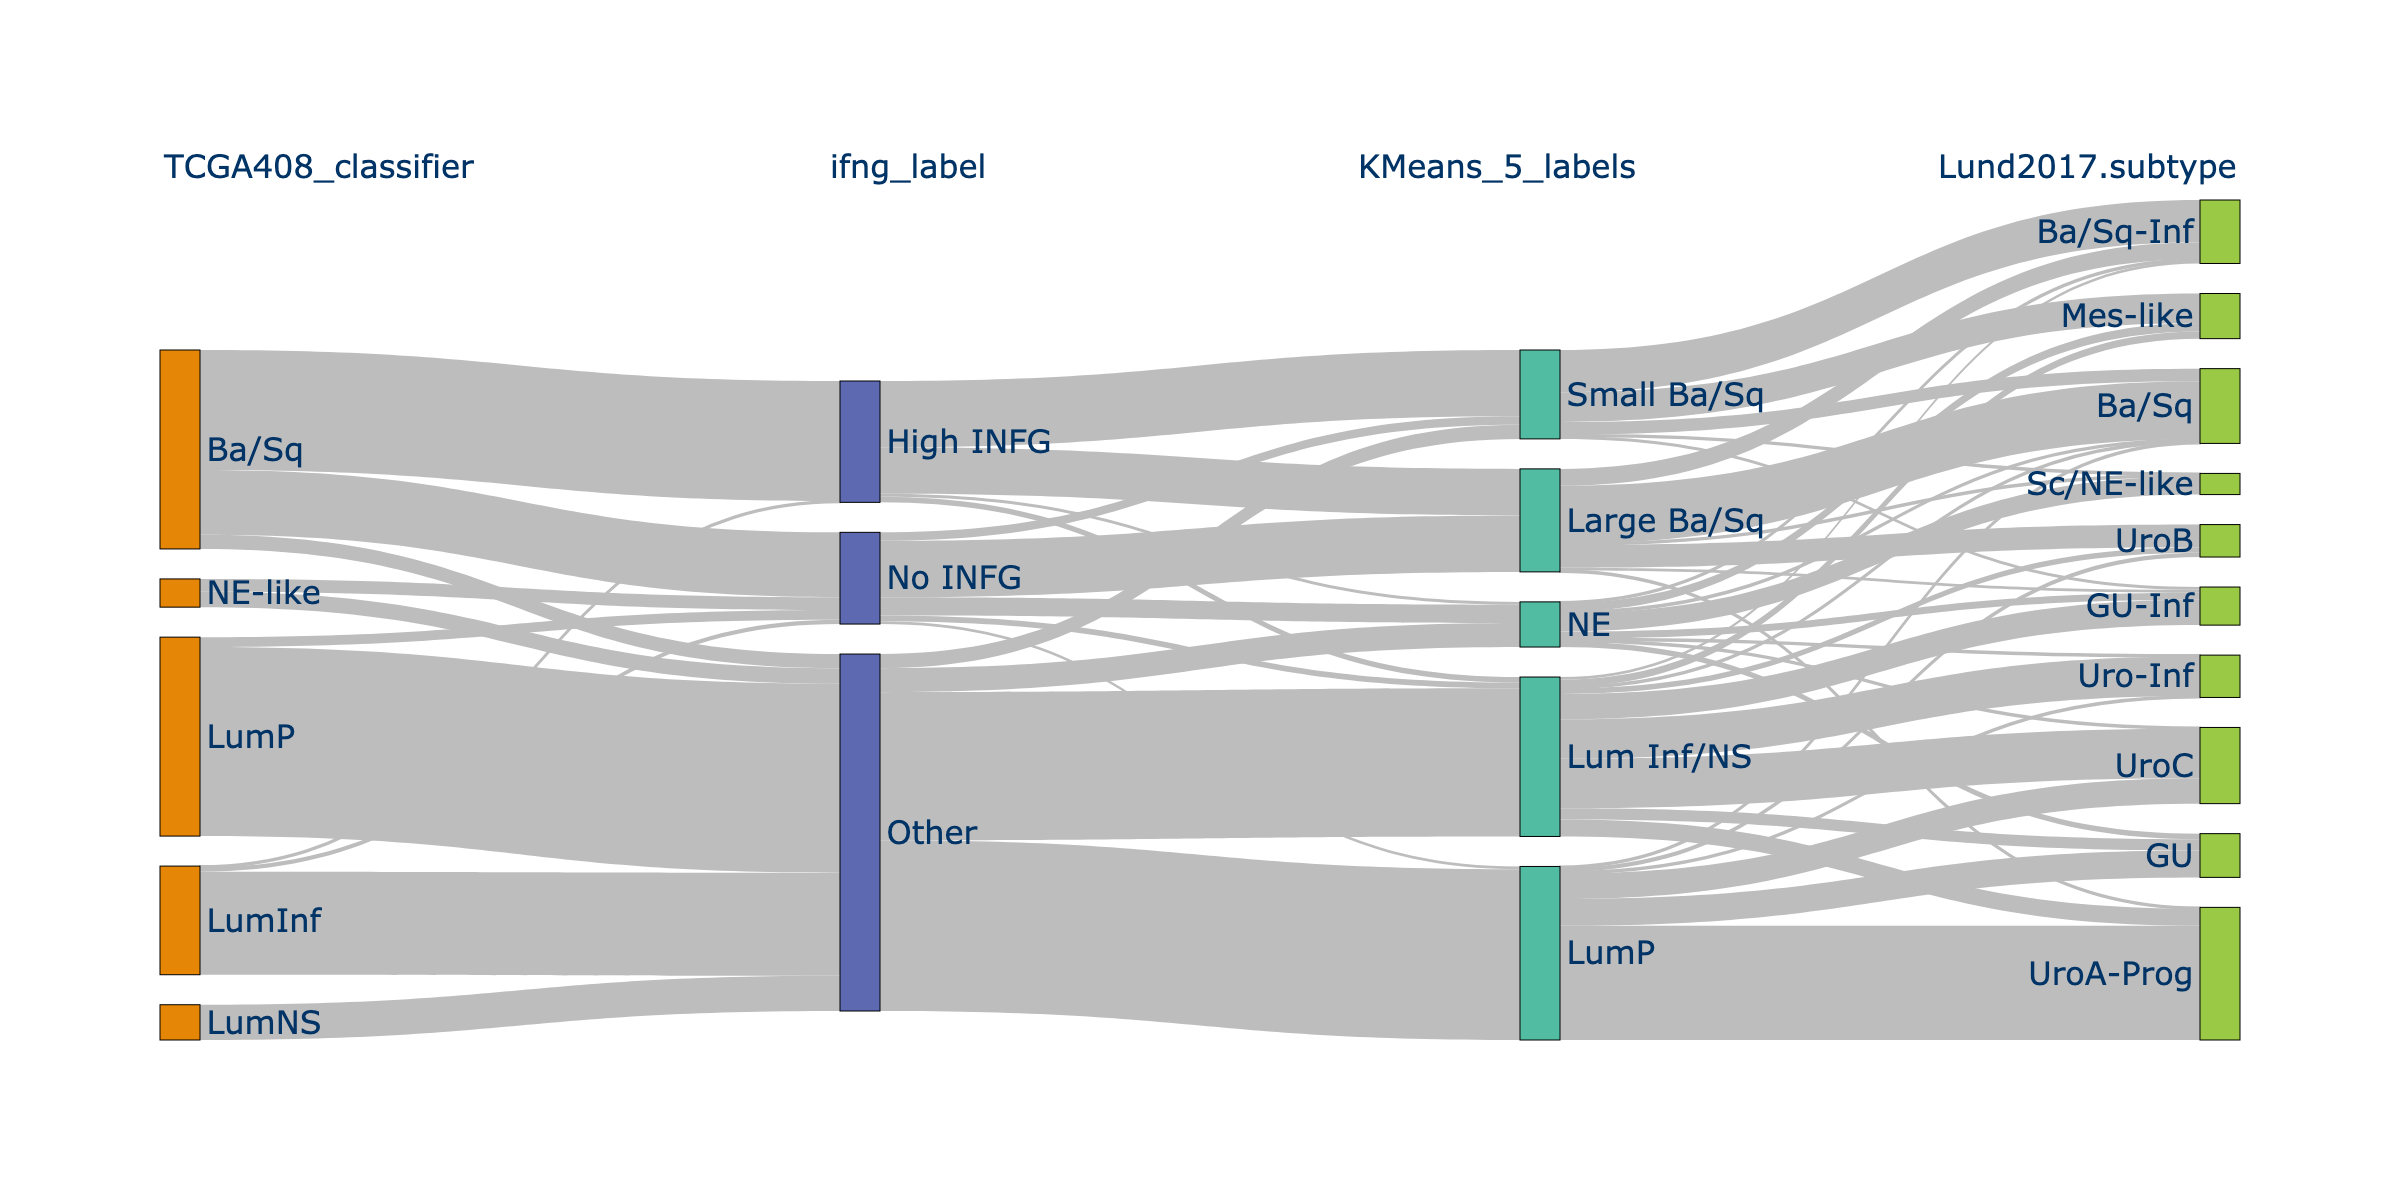
\includegraphics[width=1.0\textwidth,keepaspectratio]{Sections/ClusteringAnalysis/Resources/discussion/inf_comp.png}
        \caption{All the groups derived with K-means (K=5)}
        \label{fig:cs:ifn_all}
    \end{subfigure}
    \centering
    \begin{subfigure}[!t]{0.79\textwidth}
        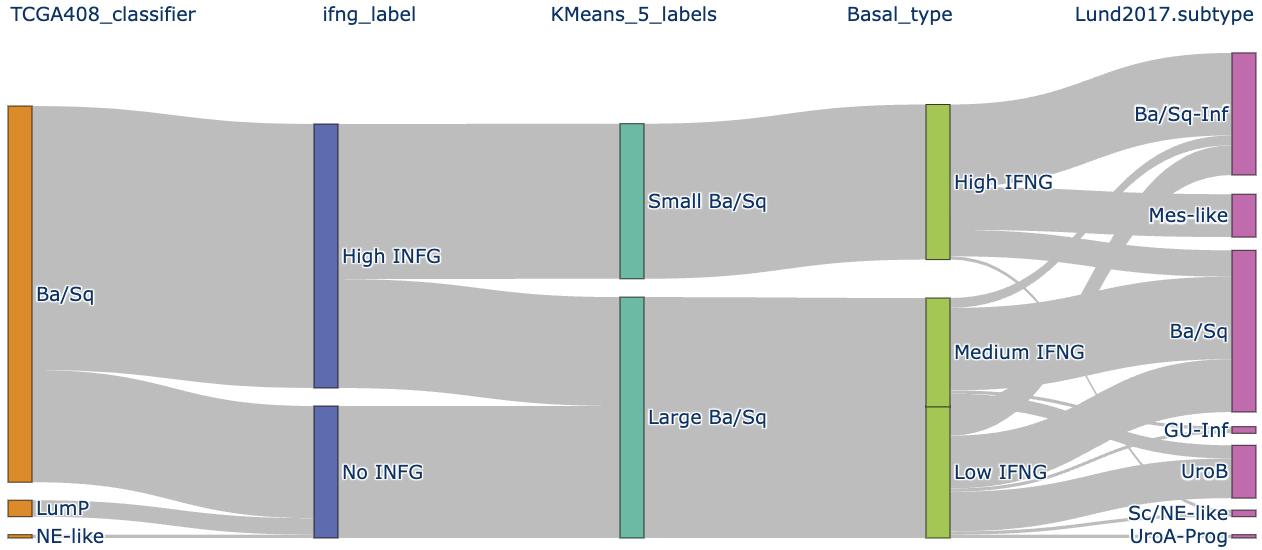
\includegraphics[width=\textwidth,keepaspectratio]{Sections/ClusteringAnalysis/Resources/discussion/inf_3_basal.png}
        \caption{Further split of the Basal group into 3 subtypes, using the work from \citet{Baker2022-bj}}
        \label{fig:cs:ifn_three_basal}
    \end{subfigure} 
    \centering
    \centering
    \caption{Sankey plot comparing the TCGA classification \citet{Robertson2017-mg}, the Interferon$\gamma$ split from \cite{Baker2022-bj}, our clustering and the Lund classifier \citet{Marzouka2018-ge}. This plot highlights that the two basal splits found through our clustering are a group of samples that have high \acrshort{ifn} (small group) and a mixed response (Large Ba/Sa). }
    \label{fig:cs:ifn_comp}
\end{figure}

% IFNG
The groups derived in this section are also compared with another work \citet{Baker2022-bj} from the Jack Birch Unit (JBU) which was focused on splitting the Basal/Squamous group by the tumour's \acrfull{ifn} response: no response and a high response. The authors identified that patients classified as high \acrshort{ifn} have a better survival prognosis compared to the ones with no immune response. In \cref{fig:cs:ifn_comp} it can be clearly seen that the Small Ba/Sq group contains a large portion of the the \acrshort{ifn} response group from \citet{Baker2022-bj}, while the large basal group a mixed of low and high \acrshort{ifn} samples. Taking the 3 main 'chords' of samples going from the \acrshort{ifn} to the Basal groups (KMeans), the Basal subtype can be further split into 3 as seen in \cref{fig:cs:ifn_three_basal}. The association of the Basal subgroups it is also supported by the Lund classifier \citet{Marzouka2018-ge}, where the Small Ba/sq (or High IFNG) contains the samples of the Ba/Sq-Inf and Mes-like from Lund, while the other two basal (in Basal\_type) are either Ba/Sq or UroB by Lund.

% Introduce the three splits
\subsubsection{Immune, Stromal and ESTIMATE score}

% Explaining the ESTIMATE score
To further validate the immune characteristics of the subgroups, the ESTIMATE score from \citet{Yoshihara2013-wq} was employed. The authors assesses tumour purity based on immune and stromal infiltration by calculating the gene expression of a subset of genes. These are known to be involved in the immune response and associated with stromal cells. The ESTIMATE, along with stromal and immune scores, were validated using DNA Copy Number Analysis and computed for the TCGA cohort.

% Check the three splits along the immune infiltration, ESTIMATE, and stroma score
The three Basal/Squamous splits, using both K-means with \( K = 5 \) and the work of \acrshort{ifn} response, can be classified into three different levels of immune response: Low, Medium, and High \acrshort{ifn} response, as seen in \cref{fig:cs:ifn_three_basal}. Across all the plots, the Y-axis is represented by the \acrshort{ifn} score from \citet{Baker2022-bj}, and the X-axis represents one of the three scores from \citet{Yoshihara2013-wq}, while the marker size is proportional to the infiltration score from the TCGA's metadata. The first scatter plot shows that High \acrshort{ifn} has the largest immune infiltration and \acrshort{ifn} response, while Low \acrshort{ifn} is at the opposite end of the spectrum, with Medium \acrshort{ifn} somewhere in between. This plot further strengthens the relationship between the Basal splits and the immune response.

\Cref{fig:cs:stroma_basal} shows the relationship between the three Basal subgroups and stromal infiltration. The spectrum is not as clear as in the previous plot, as both Low and Medium \acrshort{ifn} have a low stromal score, but the differences with the other Basal groups are clear. Lastly, the two scores are combined in the ESTIMATE scatter plot, shown in \cref{fig:cs:estimate_basal}, displaying the tumour purity of the samples in the three groups. The figure illustrates the spectrum-like nature of the Basal subtypes and their relationship, with Low \acrshort{ifn} showing the highest purity, followed by Medium and High \acrshort{ifn}, the latter being the most impure for stromal cell and immune infiltration. 



\begin{figure}[H]
    \centering
    \begin{subfigure}[!t]{1.0\textwidth}
        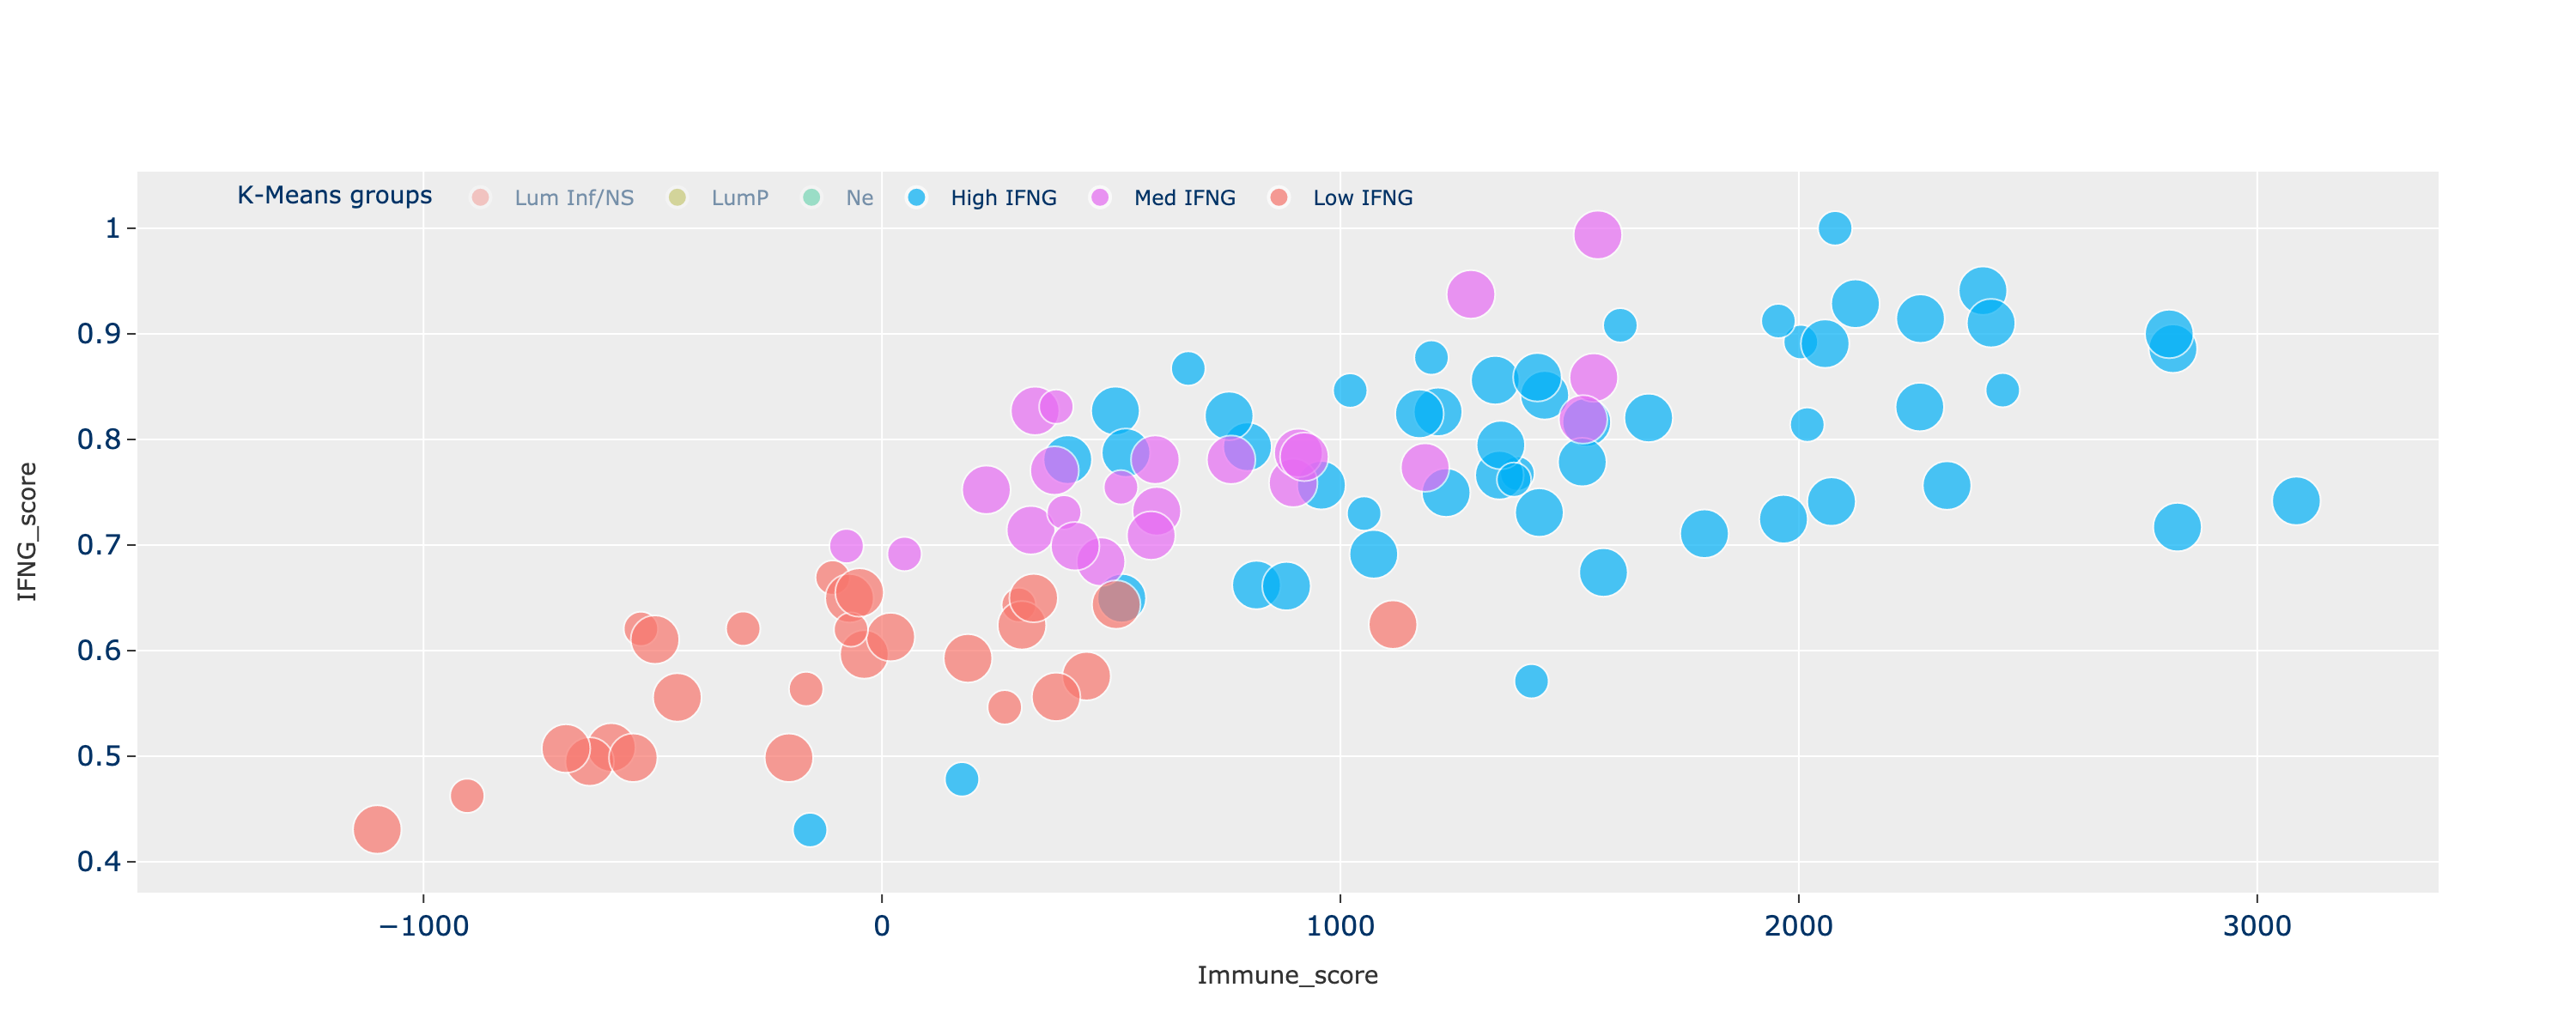
\includegraphics[width=\textwidth,keepaspectratio]{Sections/ClusteringAnalysis/Resources/discussion/Immune_spectrum.png}    
        \caption{Immune Score}
        \label{fig:cs:immune_basal}
    \end{subfigure}
    \centering
    \begin{subfigure}[!t]{1.0\textwidth}
        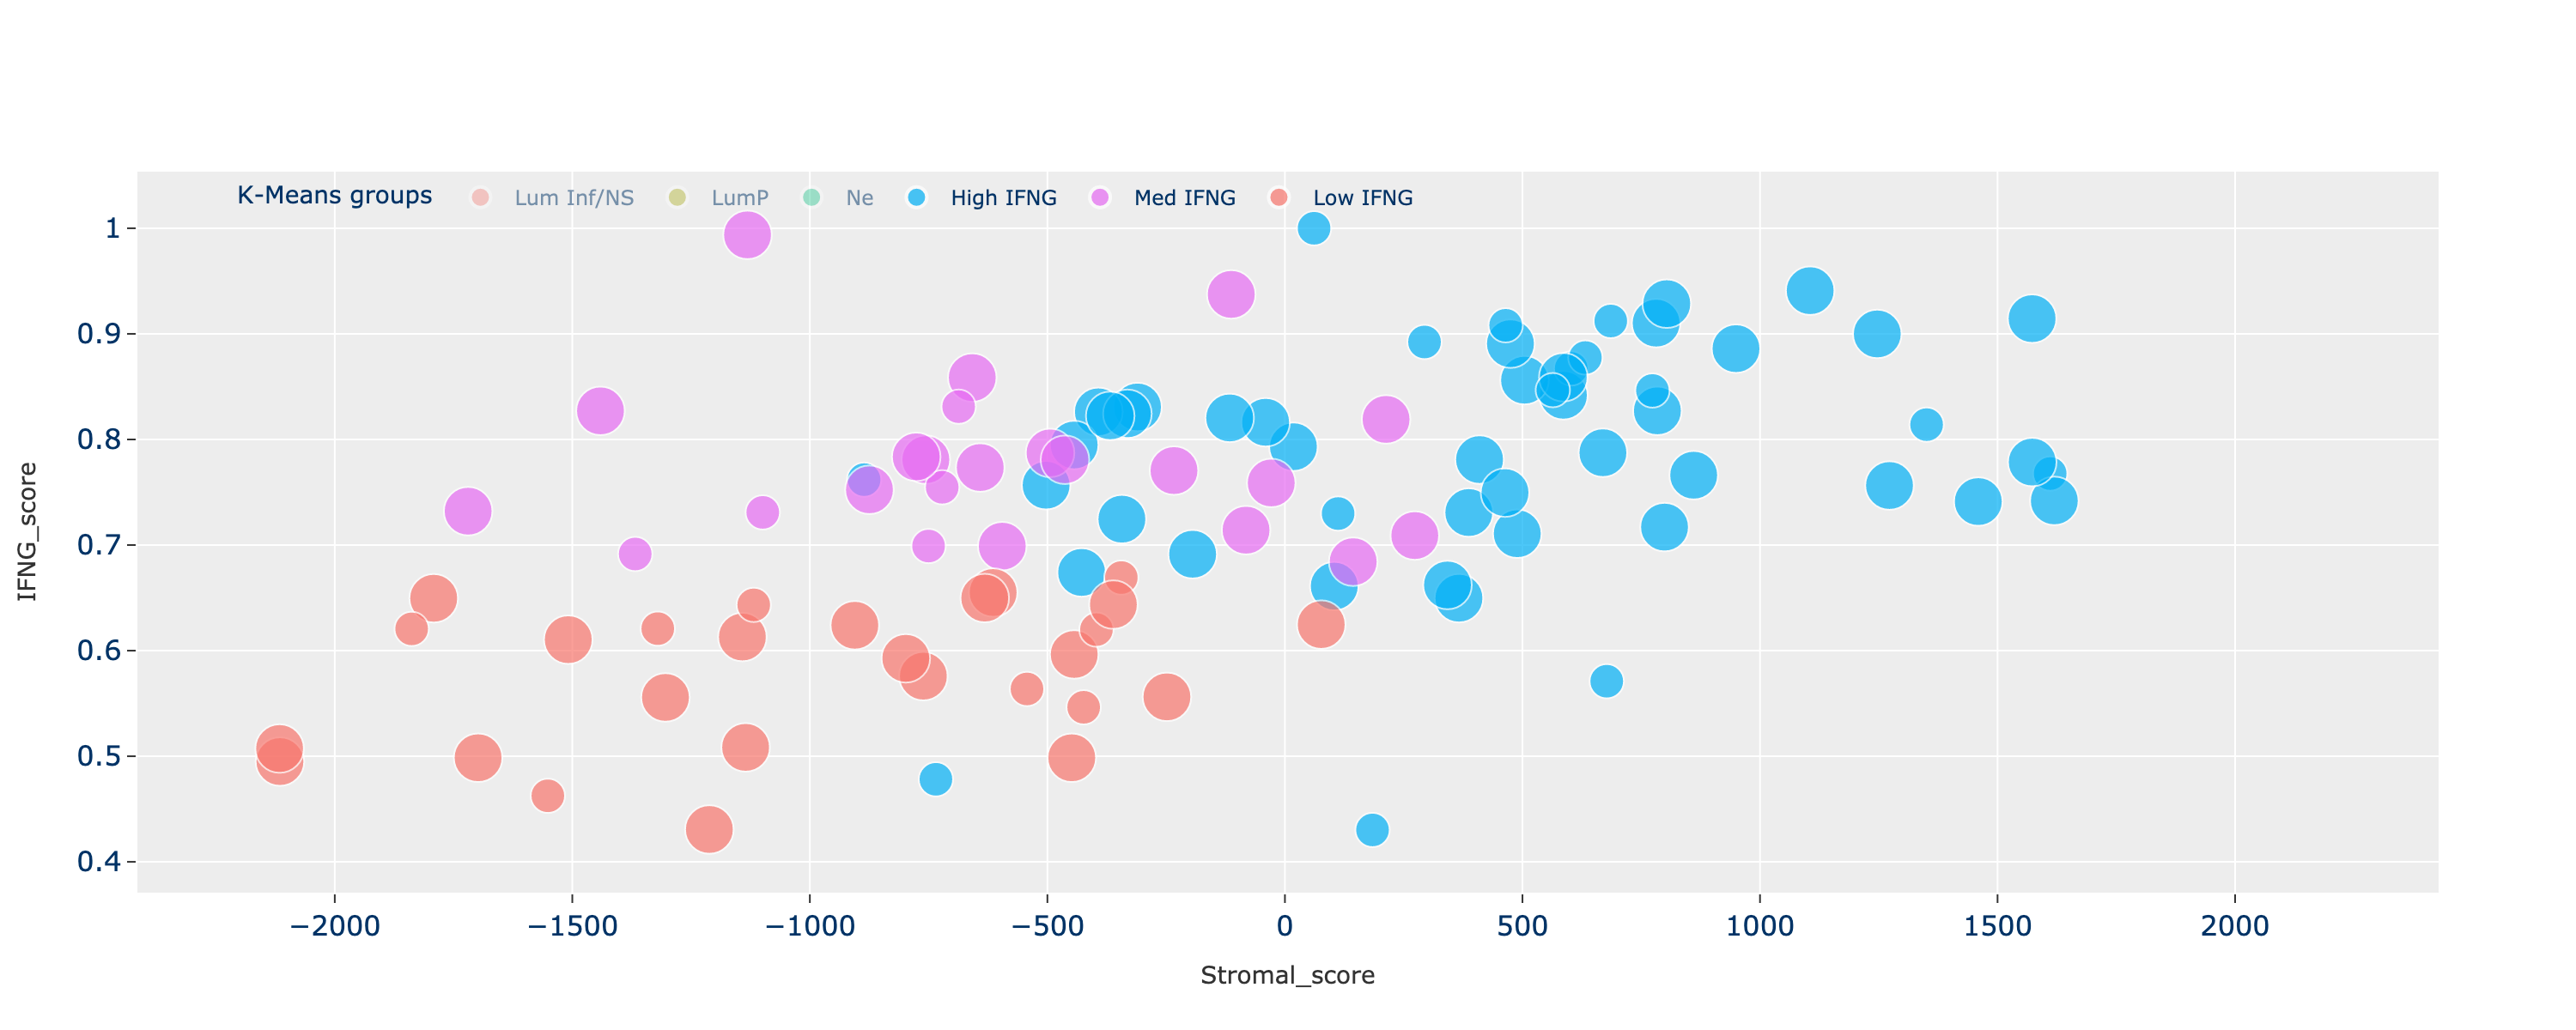
\includegraphics[width=\textwidth,keepaspectratio]{Sections/ClusteringAnalysis/Resources/discussion/Stroma_spectrum.png}
        \caption{Stroma Score}
        \label{fig:cs:stroma_basal}
    \end{subfigure} 
    \centering
    \begin{subfigure}[!t]{1.0\textwidth}
        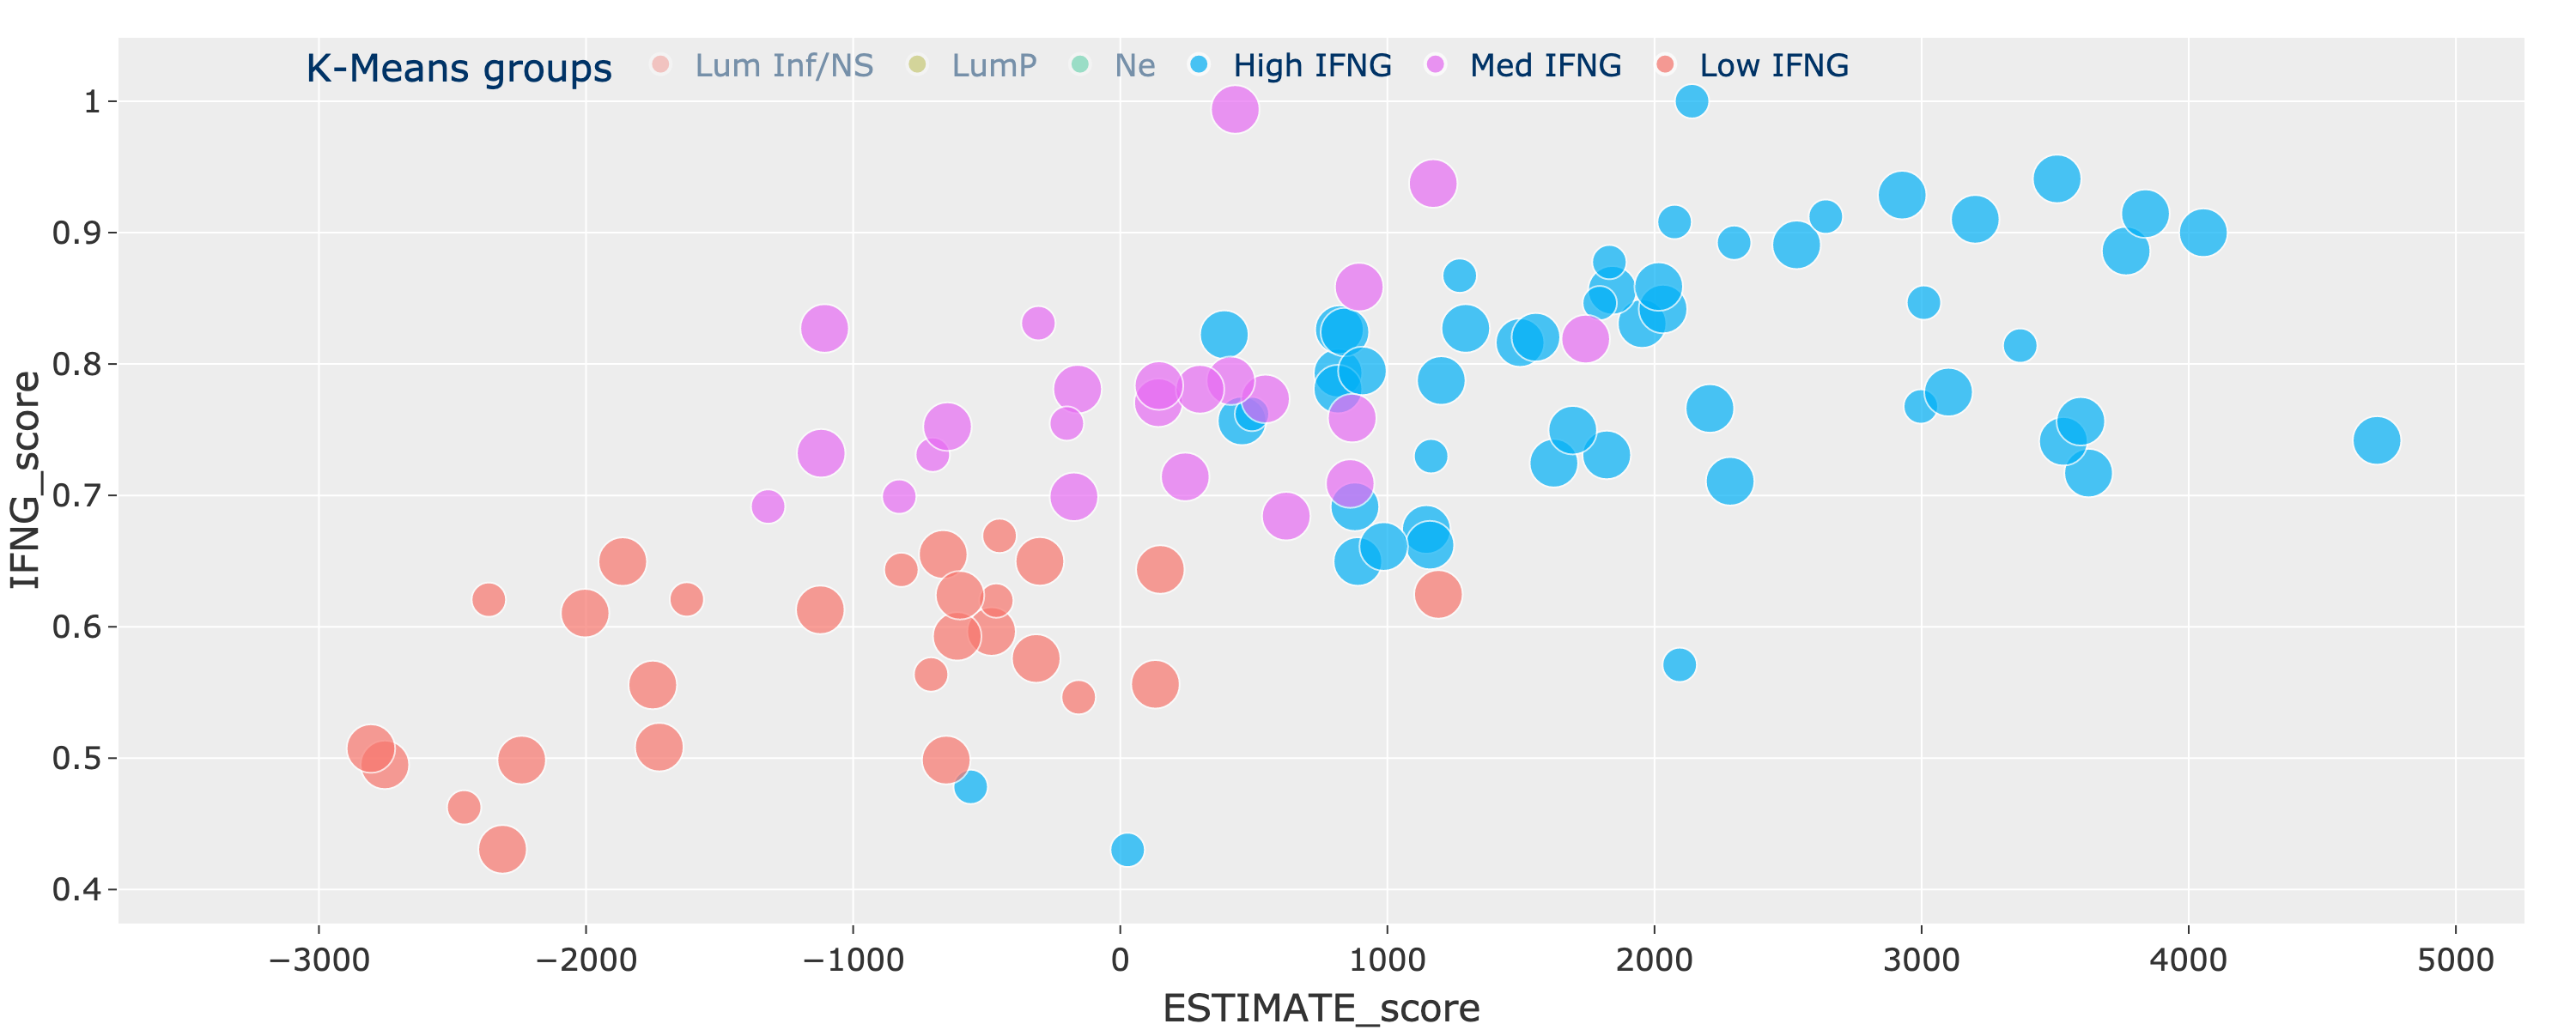
\includegraphics[width=\textwidth,keepaspectratio]{Sections/ClusteringAnalysis/Resources/discussion/Estimate_spectrum.png}
        \caption{ESTIMATE}
        \label{fig:cs:estimate_basal}
    \end{subfigure}
    \centering
    \caption{The tumour purity as indicated by the immune, stroma, and ESTIMATE scores from \citet{Yoshihara2013-wq} for the three basal splits. In all scatter plots, the Y-axis is represented by the \acrshort{ifn} score from \citet{Baker2022-bj}, the X-axis by one of the three scores, and the size of the markers is proportional to the infiltration score from \citet{Robertson2017-mg}. Positive values of the score denote infiltration by the type of cells, while negative values indicate their absence.}
    \label{fig:cs:tumour_purity}
\end{figure}


Both research Lund classification \citet{Marzouka2018-ge} and the work on \acrshort{ifn} \citet{Baker2022-bj}, split the Basal into two groups; \citet{Marzouka2018-ge} - Basal/Squamous (Ba/Sq) and Basal/Squamous infiltrated (Ba/Sq-inf) \& \citet{Baker2022-bj} - one with \acrshort{ifn} response and the other without. In each cases the two subtypes have also different survival rate where the samples with immune infiltration had a better prognosis.

The relation of the immune response and survival is also found in the Basal subgroups derived in this section, shown by performing the Kaplan-Meier survival analysis shown in \cref{fig:cs:basal_survival}. The figure displays the Basal group
from \citet{Robertson2017-mg} by the green line, and the other 3 lines are represented by the subtypes found in this section. From the survival rates it can be noticed how the 3 basal groups constitute the TCGA's Ba/Sq group and that the poorest prognosis is given by the Low IFNG samples. This plot shows the importance of improving the MIBC classifications. 


\begin{figure}[!htb]    
    \centering
    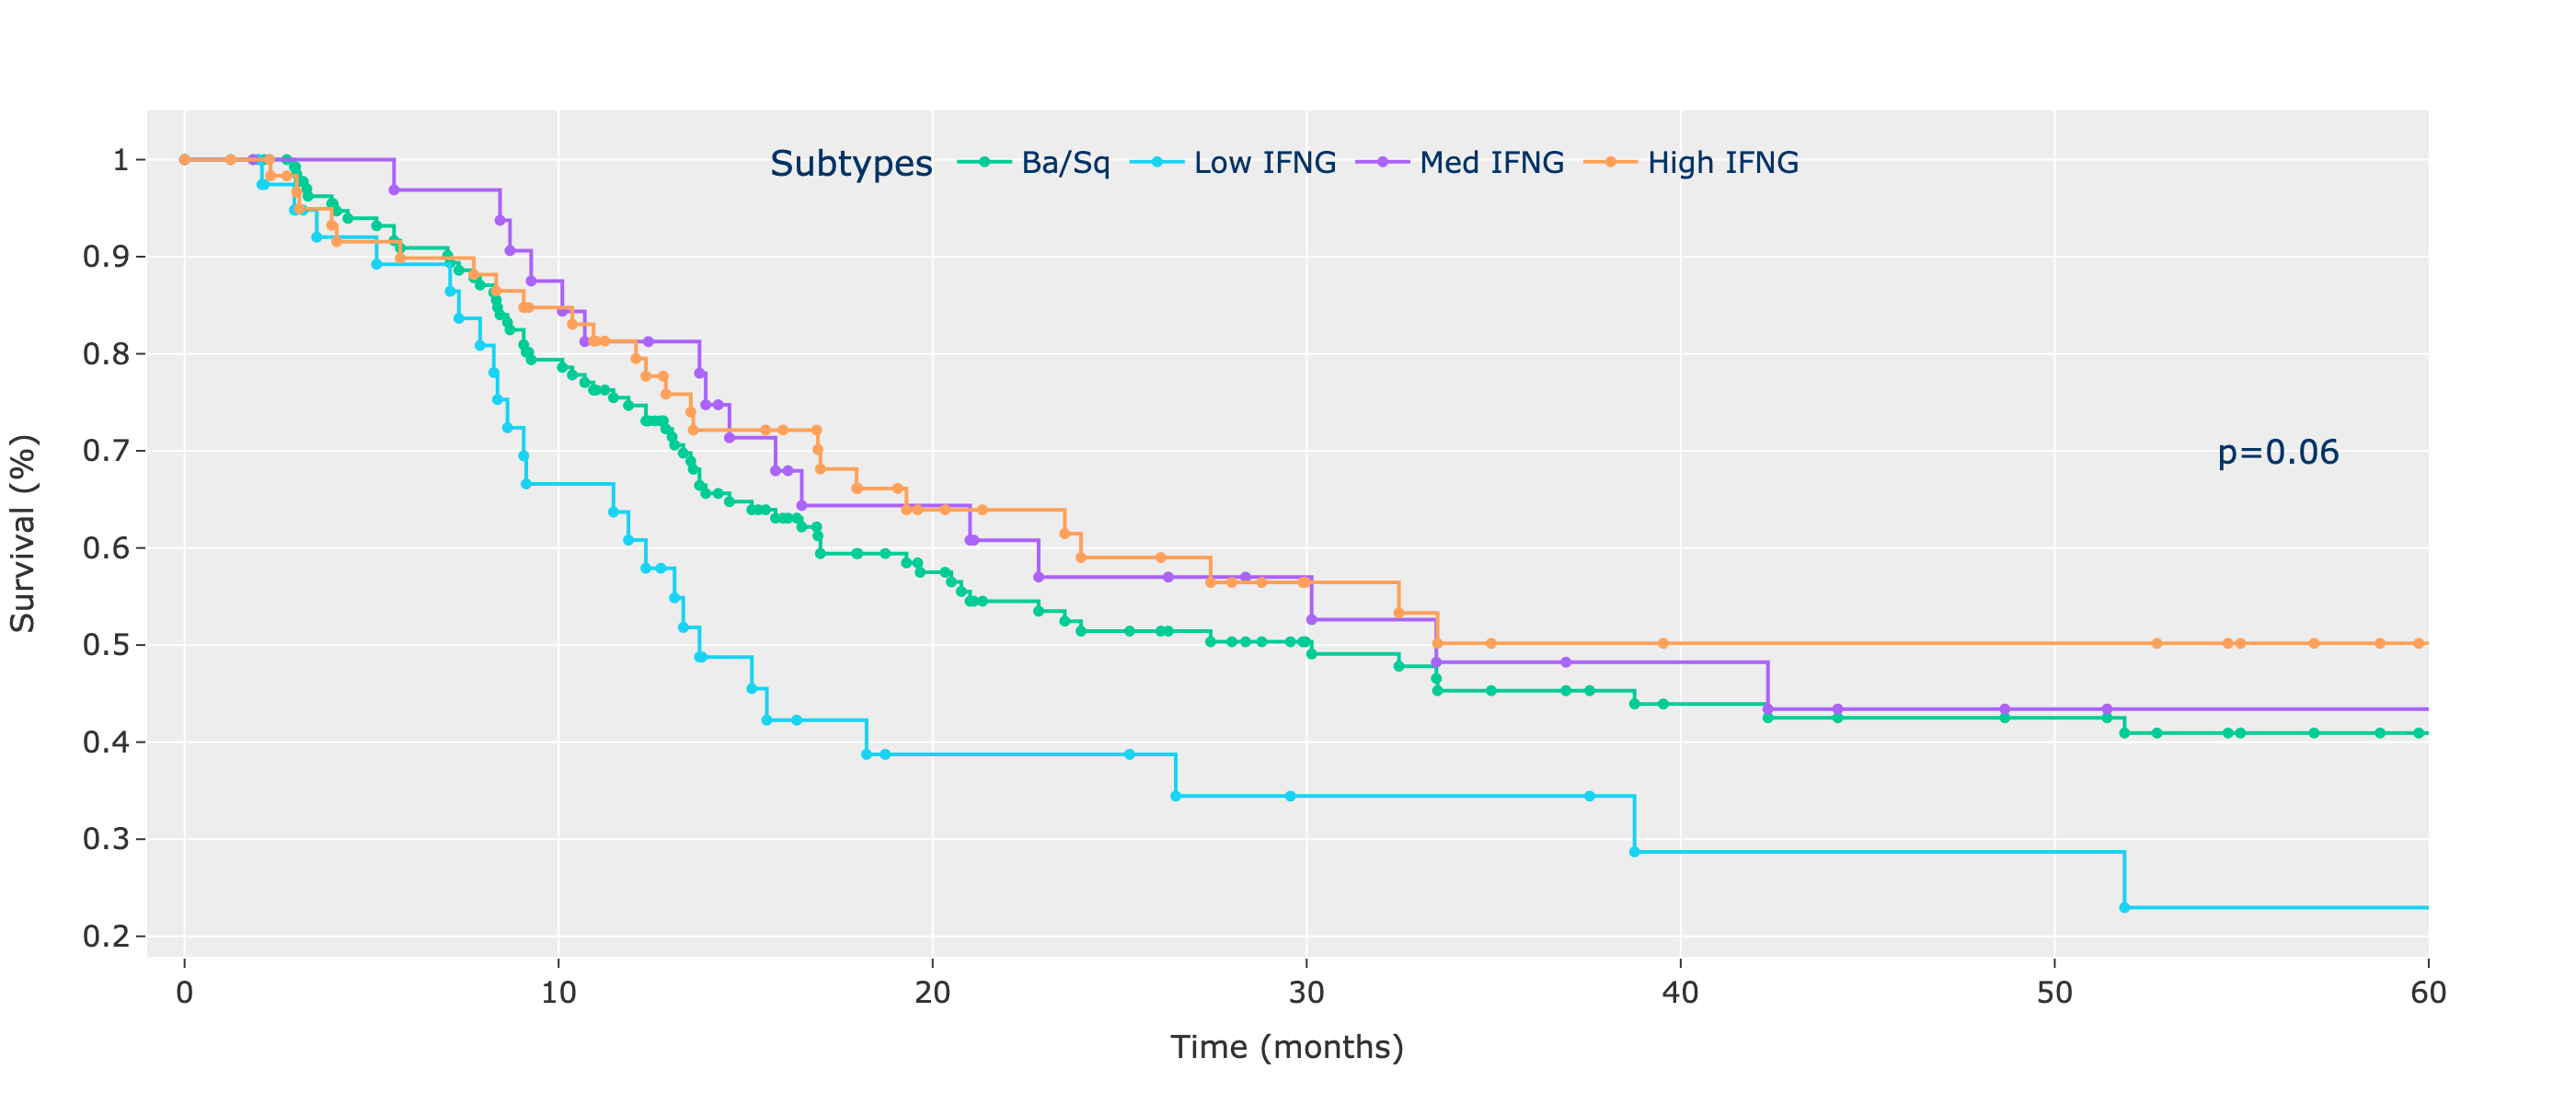
\includegraphics[width=1.0\textwidth,keepaspectratio]{Sections/ClusteringAnalysis/Resources/discussion/survival_basal.png}
    \caption{Kaplan-Meier survival analysis of the 3 Basal groups derived in \cref{s:cs:bio_interp} using K-means with K=5 and the basal subgroups by the \acrshort{ifn} response \citet{Baker2022-bj}, and the Ba/Sq survival from TCGA classification \citet{Robertson2017-mg}.}
    \label{fig:cs:basal_survival}
\end{figure}

\subsubsection{Basal exploration} \label{s:cs:basal_interp}

Differential Expression Analysis (DEA) was employed to further explore the subgroups derived among the MIBC subtypes. The focus was particularly on the Basal groups, as the three-way split introduced novel aspects, some of which had been previously validated through other classifications \citet{Baker2022-bj,Marzouka2018-ge}.

% Intro to pi plots
To delve deeper into the molecular characteristics, the Pi scatter plot is utilised as shown in \cref{fig:cs:pi_basal}. This figure integrates two distinct DEAs, with one represented on each axis, by calculating the pi values as outlined in \cref{s:cs:pi_val}. Here, the $q-value$ represents the significance of the expression difference as determined by sleuth, and the $FC$ denotes the fold-change between the two compared groups. Consequently, the pi-values encapsulate both the gene difference and its statistical significance.


\begin{equation} \label{s:cs:pi_val}
    pi = - log_{10}(q_{val}) * log_{2}(FC)
\end{equation} 

% Low IFNG
The Low IFNG group has the poorest survival prognosis making it the focus of the Basal comparisons. The Pi-plot in \cref{fig:cs:pi_basal} contrasts the Low IFNG with the MED IFNG on the Y-axis and the Low IFNG with the High IFNG on the X-axis. The initial observation from the scatter plot is the sparse presence of markers in the quadrant specific to Low IFNG, indicating that few genes distinctly characterise Low IFNG in comparison to the other Basal subtypes. This is specifically highlighted by the small scale of the Y-axis, where the Med and Low IFNG are compared, showing \textit{GSTM3} as being distinct for the latter.

On the X-axis, which highlights the genes unique to Low IFNG over High IFNG, several known squamous markers such as \textit{ZBTB7C, TP64, DSC3} are present. Notably, \textit{FGFR3}, a well-documented differentiation-associated marker and extensively studied gene in MIBC, is also positioned on the X-axis.

\begin{figure}[!htb]
    \centering
    \begin{subfigure}[!t]{1.0\textwidth}
        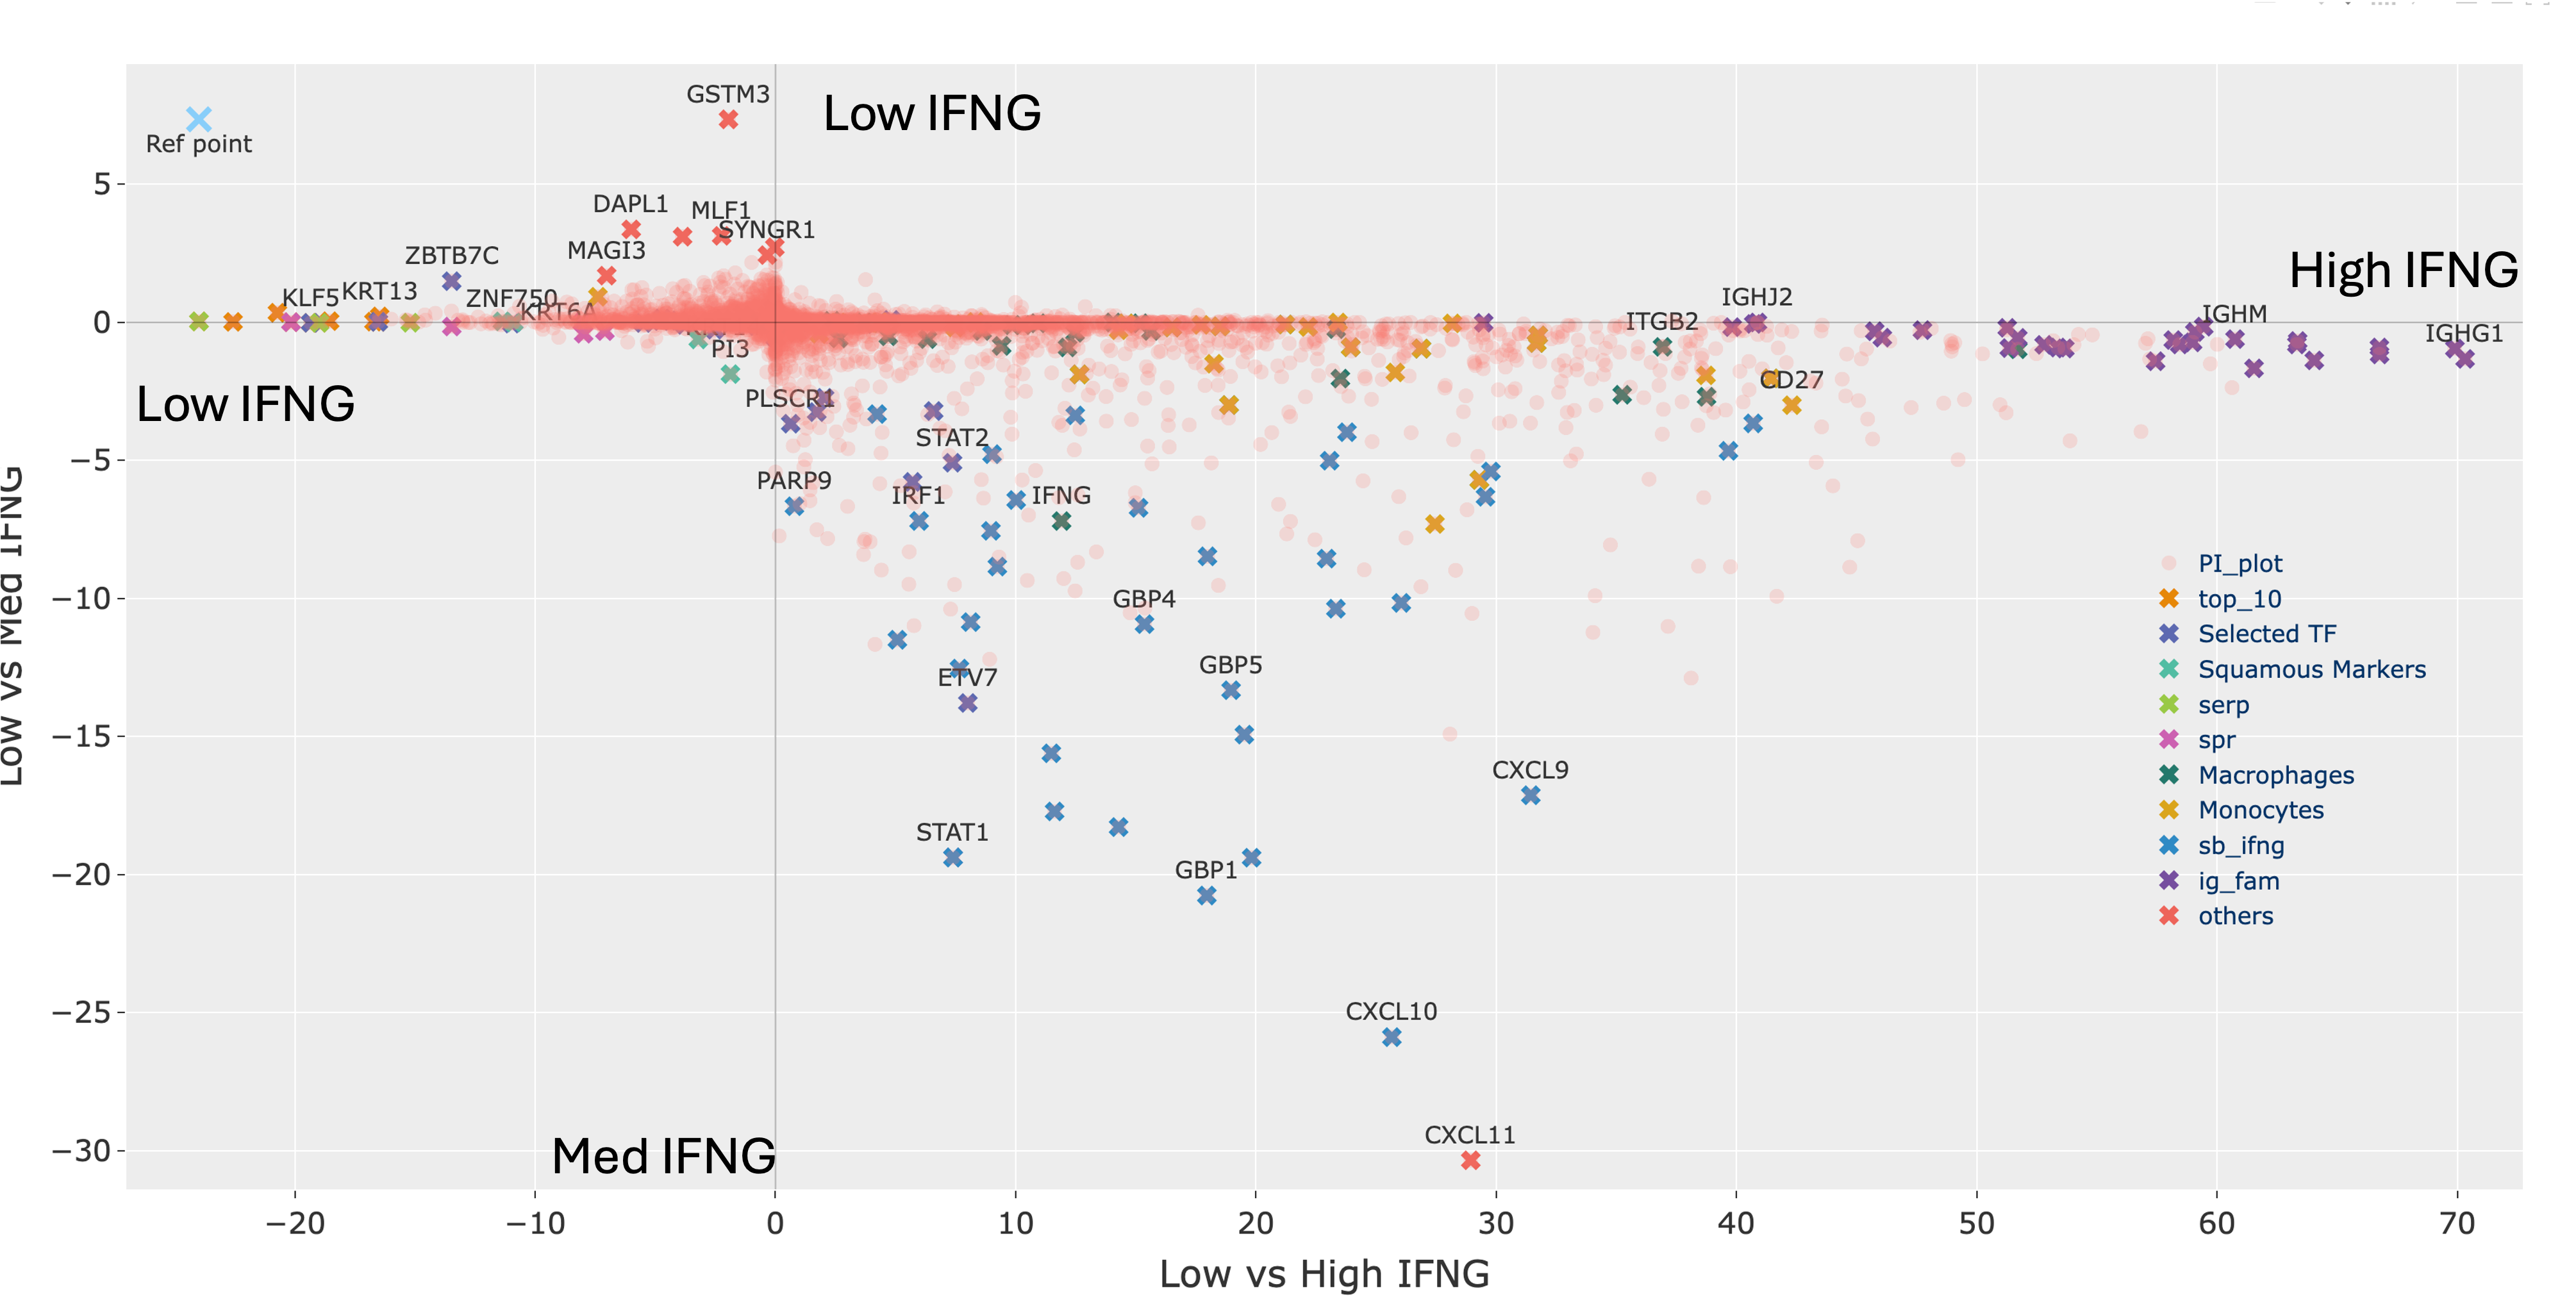
\includegraphics[width=\textwidth,keepaspectratio]{Sections/ClusteringAnalysis/Resources/discussion/basal_comp_pi.png}    
        \caption{Basal comparison}
        \label{fig:cs:basal_comp}
    \end{subfigure}
    \centering
    \begin{subfigure}[!t]{1.0\textwidth}
        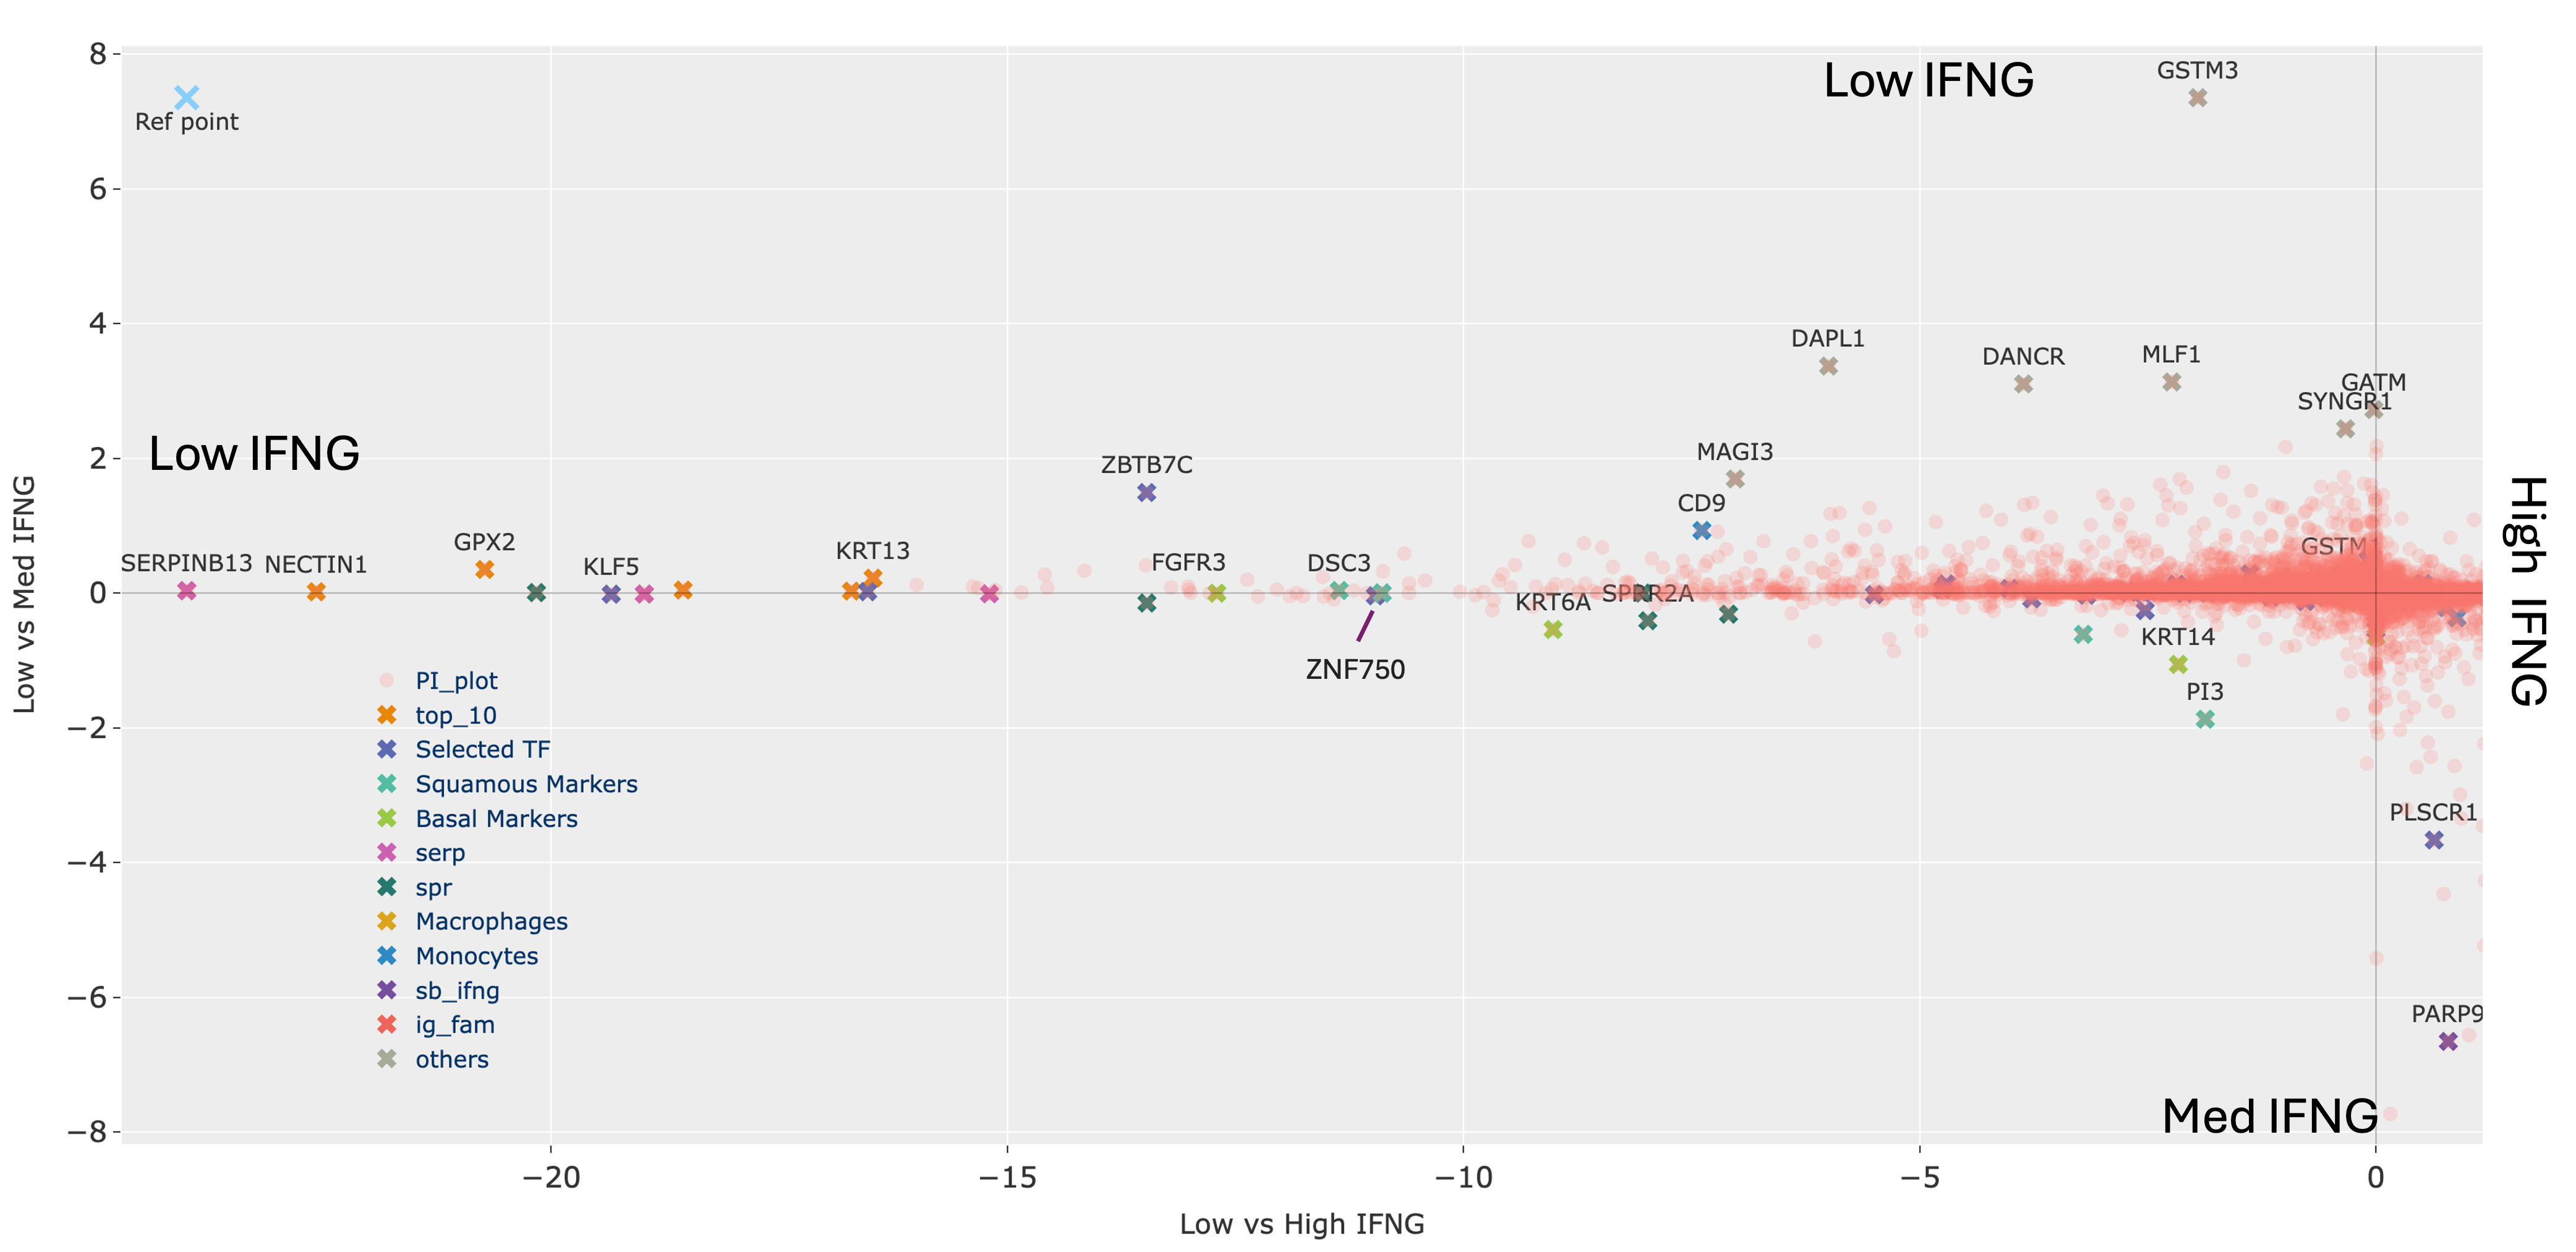
\includegraphics[width=\textwidth, keepaspectratio]{Sections/ClusteringAnalysis/Resources/discussion/basal_comp_pi_zoom.png}
        \caption{Basal comparison zoom in}
        \label{fig:cs:basal_comp_zoom}
    \end{subfigure} 
    \centering
    \caption{Pi plot showing the two DEA run, on the X-axis: the Low vs High IFNG and on the Y-axis: the Low vs Med IFNG.} 
    \label{fig:cs:pi_basal}
\end{figure}


% Unknown genes
Some of the genes, \textit{DANCR, DAPL1, GATM, GSTM3, MLF1, SYNGR1, GSTM1, MAGI3}, positioned on the positive side of the Y-axis and labelled as 'other', were not classified by any of the 'known markers'. However, some of these genes play a role in bladder or other cancers. In an \textit{in-vitro} study by \citet{Zhan2018-um}, \textit{DANCR} (or \textit{ANCR}), a long non-coding RNA (lncRNA), was found to play an oncogenic role in bladder cancer\footnote{There is a review by \citet{Wang2021-gn} on the role of \textit{DANCR} in bladder and other cancers.}. According to a review by \citet{Li2023-mk}, which focused on \textit{MLF1}, this gene may be involved in various types of cancer, including bladder cancer, and could influence the immune response. \textit{GATM} is suggested to be a tumour suppressor gene that influences a type of metastatic renal cancer, as indicated in a transcriptomic study by \citet{Jee2022-wi}. \textit{GSTM3} and \textit{GSTM1} are known to be genetic risk factors for bladder cancer \citet{Schnakenberg2000-cu}. The roles of \textit{MAGI3, MLF1,} and \textit{DAPL1} are less well-known.

% Specific to the low over the high 
In \cref{fig:cs:basal_comp_zoom}, on the negative side of the horizontal axis, it ca be seen the markers that are significantly differently expressed in the Low IFNG over the High IFNG group. Most of the genes are Squamous/Basal markers.

% High IFNG and MEDIUM 
In the diagonally opposite quadrant (II) are genes involved in both High and Medium IFNG Basal groups, which contain considerably more markers than the Low IFNG's quadrant. On the positive X-axis, most of the genes are part of the Immunoglobulin family (\textit{IG-}), and are associated with macrophages and monocytes, all known to be related to the immune response. This confirms that High IFNG is the strongest Basal subgroup associated with the immune response. The \acrshort{ifn} response markers from \citet{Baker2022-bj} are enriched in both Med and High IFNG subtypes, as shown by the purple markers.


% Introduce the other plot
To further investigate the relationship of the Basal groups with the immune response of the tissue, another Pi plot was utilized in \cref{fig:cs:pi_basal_inf}. The Y-axis displays the Pi values generated from the DEA of Low IFNG versus Luminal Infiltrated, while the X-axis represents the DEA between High and Med IFNG subgroups. In this analysis, Low IFNG is considered the MIBC subtype with the least immune response, whereas Lum INF is regarded as a non-basal group with high immune infiltration. This scatter plot thus elucidates the tendencies of the three Basal subtypes.

% High IFNG
The first quadrant contains markers that are specific to both the LumInf and the High IFNG groups. It is evident that the family of immunoglobulin genes is common to both groups. On the positive X-axis, there are many markers for other immune-related responses, such as B and T cells, as well as monocytes and macrophages. This further reinforces the immune characteristics previously observed for High IFNG and highlights the stronger immune response of High IFNG compared to Med IFNG.


\begin{figure}[!htb]    
    \centering
    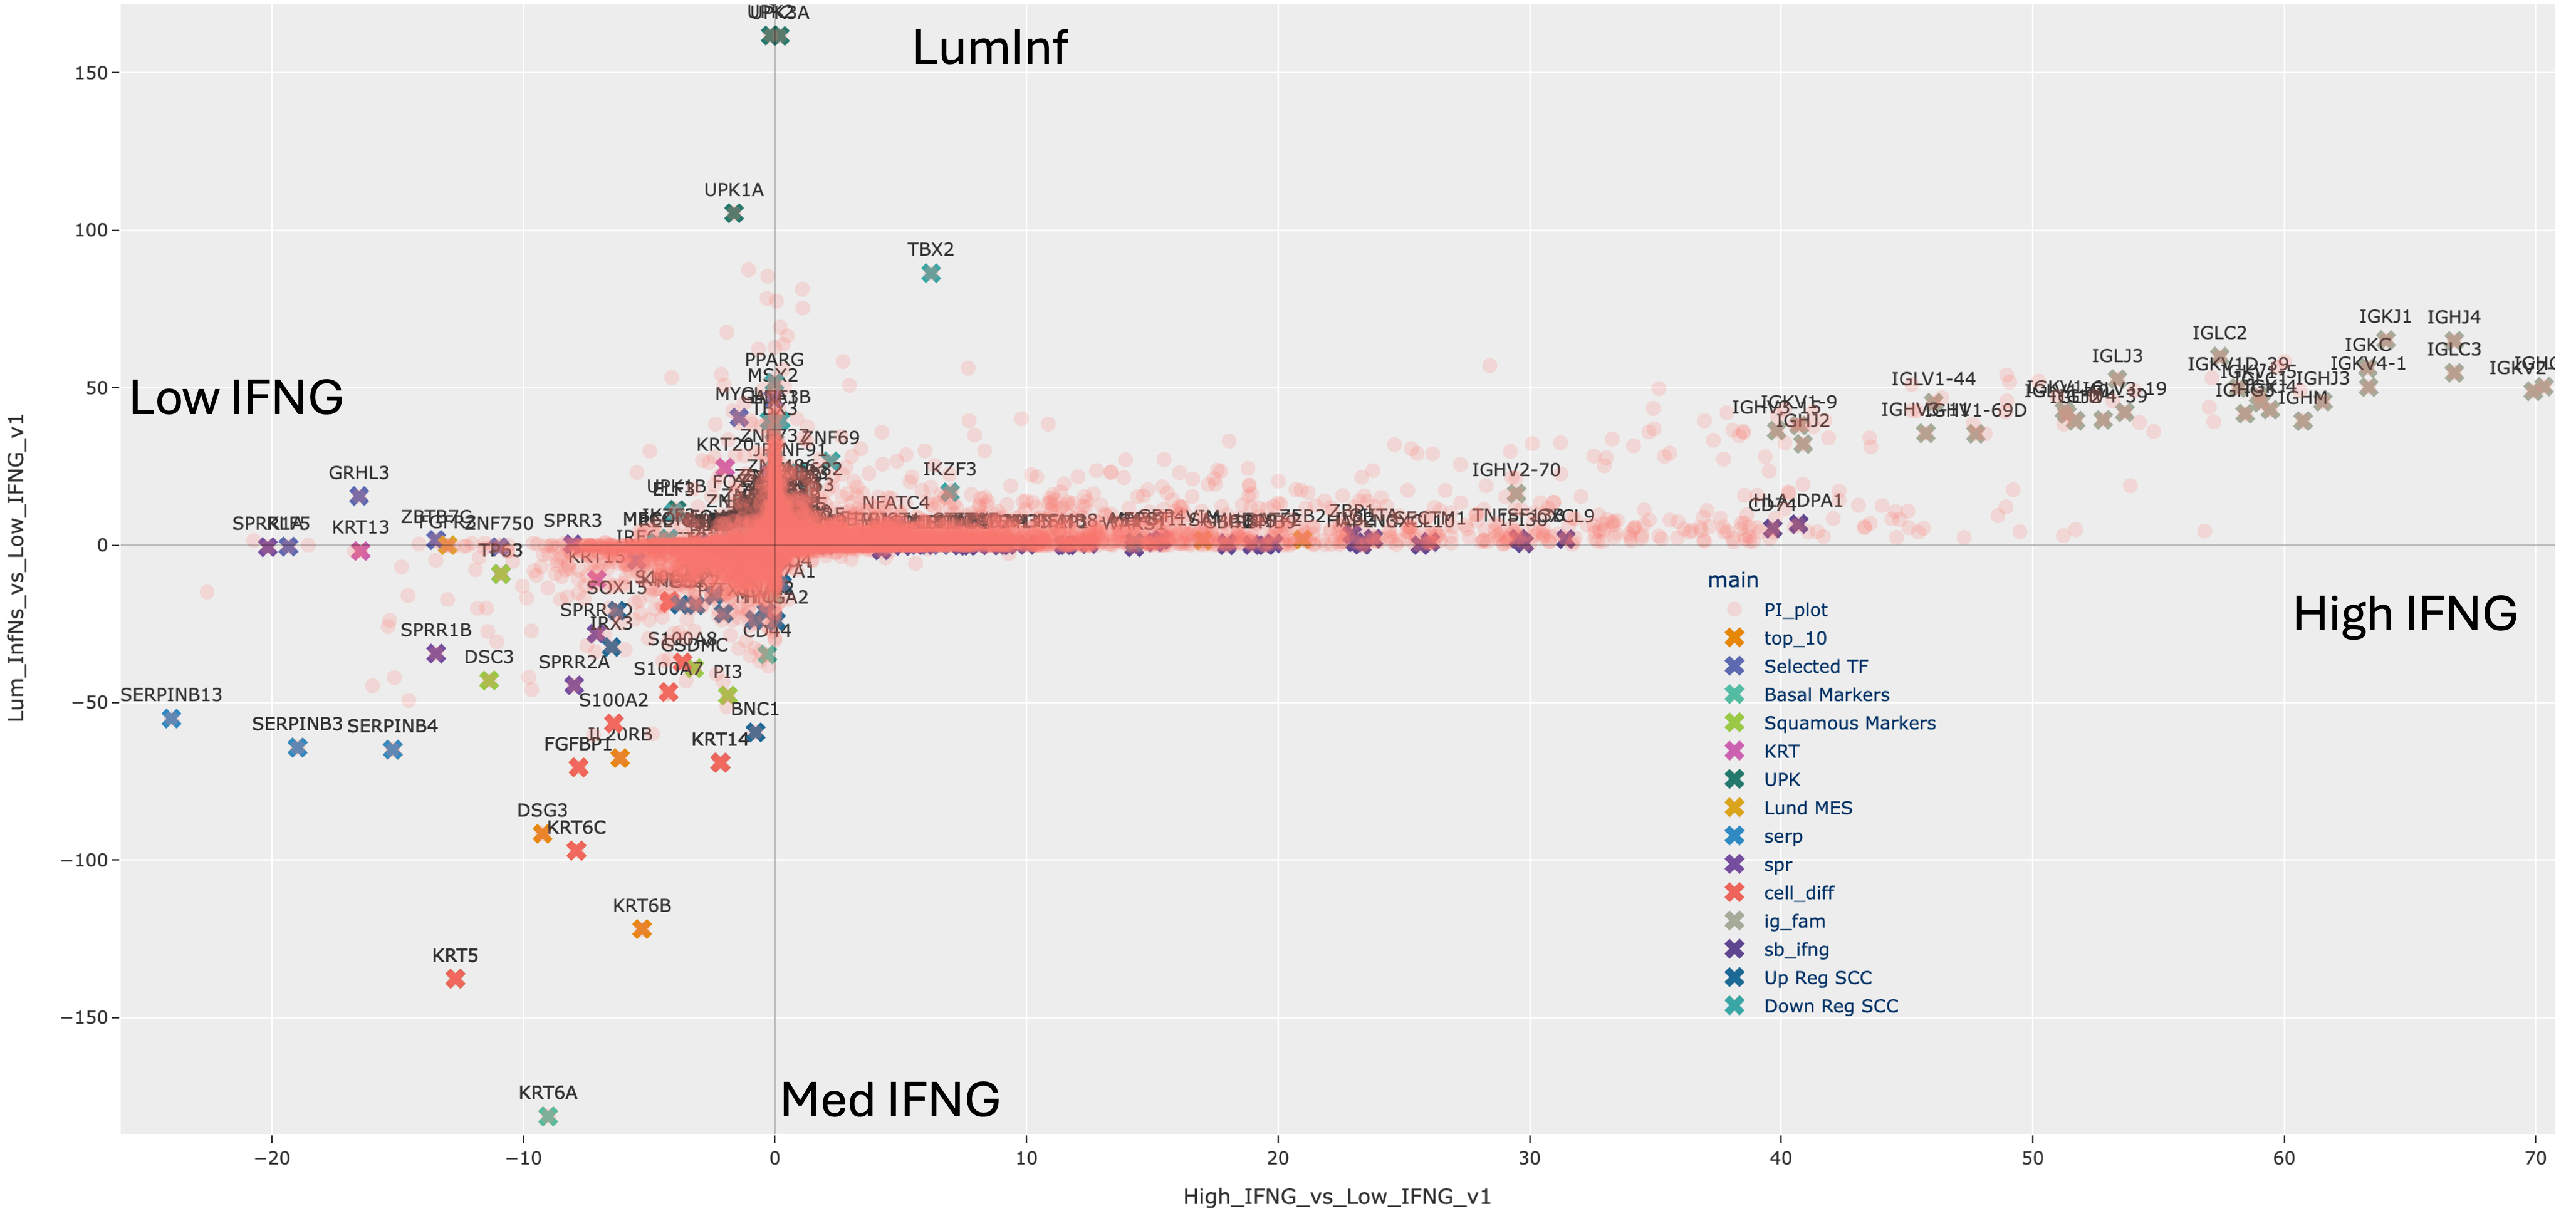
\includegraphics[width=1.0\textwidth,keepaspectratio]{Sections/ClusteringAnalysis/Resources/discussion/basal_inf_pi.png}
    \caption{Pi plot showing the two DEA run, on the X-axis: the Med vs High IFNG and on the Y-axis: the Luminal Infiltrated vs Low IFNG. }
    \label{fig:cs:pi_basal_inf}
\end{figure}


% Medium and LumInf
It can be observed that there are fewer common genes between the Med IFNG and the LumInf in the fourth quadrant. Some of the genes on the negative side of the Y-axis, which are specific to Med IFNG over High IFNG, are involved in squamous or basal tissue, such as \textit{ZBTB7C, ZNF750, KRT13, \textbf{KLF5}, SPRR1A}. The genes specific to Ba/Sq are even more prevalent in the third quadrant, between Low and Med IFNG, where many of the common genes are well-known squamous or basal markers: \textit{DSC3, KRT6A, KRT5, TP63}, and the \textit{SERPIN} and \textit{SPR} families.

The two figures \cref{fig:cs:pi_basal,fig:cs:pi_basal_inf} further reinforce the existence of three distinct immune responses by the basal tumours. They highlight the genes specific to each subtype, where High IFNG exhibits very specific immune responses, even compared to the LumInf subgroup. Med IFNG is positioned between a high immune response and no response, as seen in the samples from Low IFNG. Basal and squamous markers are evident in both Low and Med IFNG groups, as clearly demonstrated in \cref{fig:cs:pi_basal_inf}, and are also supported by the ESTIMATE scores in \cref{fig:cs:tumour_purity}.



\subsubsection{LumInf} \label{s:cs:lumInf_interp}

The previous subsections were focused on understanding the molecular properties of the Basal subgroups, identifying High IFNG to be 'closer' to the Luminal infiltrated. To elucidate the molecular particularities of the luminal infiltrated groups, the Pi-plot was constructed using the DEA results from LumInf versus Low IFNG on the X-axis and LumInf versus LumP on the Y-axis. The Low IFNG group was chosen as a representative of the Basal groups as it lacks immune infiltration, thereby highlighting the LumInf properties, while LumP was selected to examine shared luminal features.

% Introducing GSEA
\acrfull{gsea} was run on the REACTOME (see \cref{fig:cs:ne_gsea}) and Hallmarks (see \ref{fig:ap:cs:gsea_ne_hallmark}) database using GSEApy \citet{Fang2023-ec} package. The ranking was computed by using the referential point in quadrant II (see light blue cross in \cref{fig:cs:lumInf_gsea}) representing the point with the 'strongest' LumInf molecular properties across the two DEA comparisons; this is determined by the maximum point on the X-axis and the minimum on the Y-axis. The distance to all the other points from the referential marker are computed, which are then ranked. This method is widely used in this PhD project as it provides a ranking system in the context of two DEA, focusing on the genes specific to a quadrant, in this case the LumInf. 

% Commenting the immune aspect of the Pi plot
The striking group of points in the second quadrant of \cref{fig:cs:lumInf_pi}, specific to LumInf, includes the immunoglobulin family, denoting the immune infiltration characteristic of the group. This is further substantiated by the results from the GSEA in \cref{fig:cs:lumInf_gsea}, where most pathways found in Reactome involve genes linked to the immune response, such as \textit{FCGR Activation}, \textit{CD22 mediated BCR regulation}, or \textit{creation of C4 and C2 activators}.


% Positive on the X-axis showing the luminal characteristic
The positive values on the X-axis shows genes that are differentially expressed in LumInf compared to the Low IFNG group and exhibit a luminal-like aspect. These markers include genes known as luminal markers, such as \textit{UPK1A, UPK3A, UPK2, PPARG, GATA3}, confirming the luminal characteristics of the subtype. The negative values on the X-axis are Basal-specific markers, such as \textit{KRT6A} and \textit{KRT5}. The lack of scatter points and the small scale of the Y-axis indicate that the Luminal Infiltrated and Luminal Papillary groups do not share many genes.

This analysis confirms both the immune infiltration and the luminal molecular characteristics of the LumInf group, derived using the methods presented in this section.

\begin{figure}[H]
    \centering
    \begin{subfigure}[!t]{1.0\textwidth}
        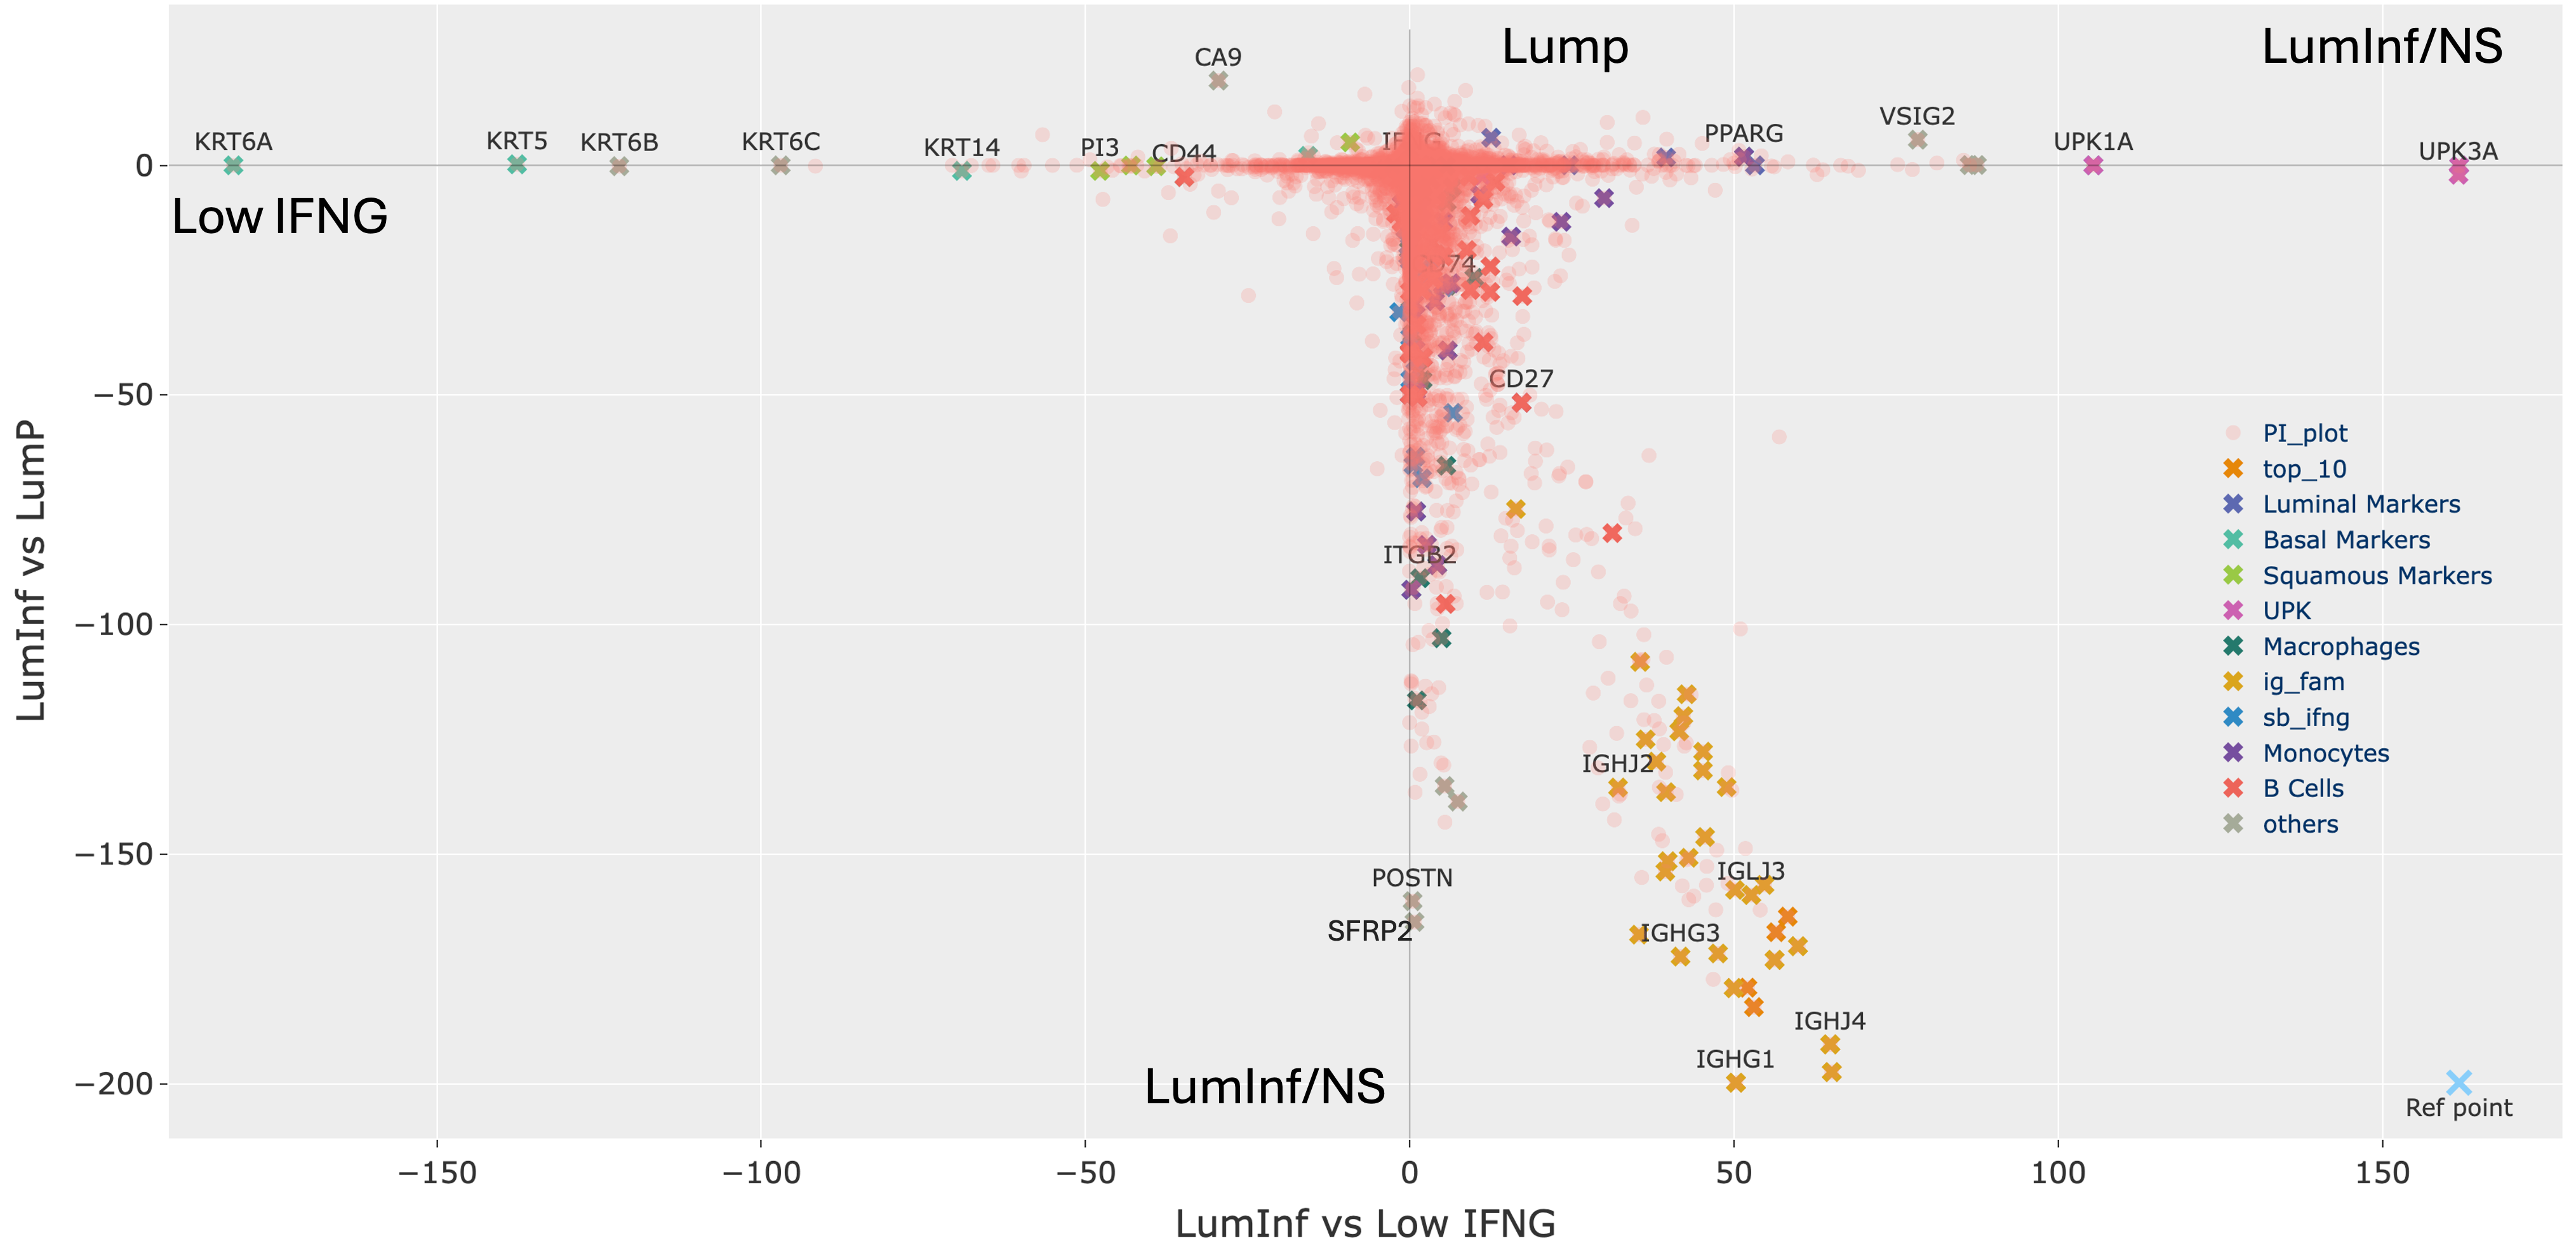
\includegraphics[width=\textwidth,keepaspectratio]{Sections/ClusteringAnalysis/Resources/discussion/other_groups/lumInf_pi.png}    
        \caption{Pi}
        \label{fig:cs:lumInf_pi}
    \end{subfigure}
    \centering
    \begin{subfigure}[!t]{0.9\textwidth}
        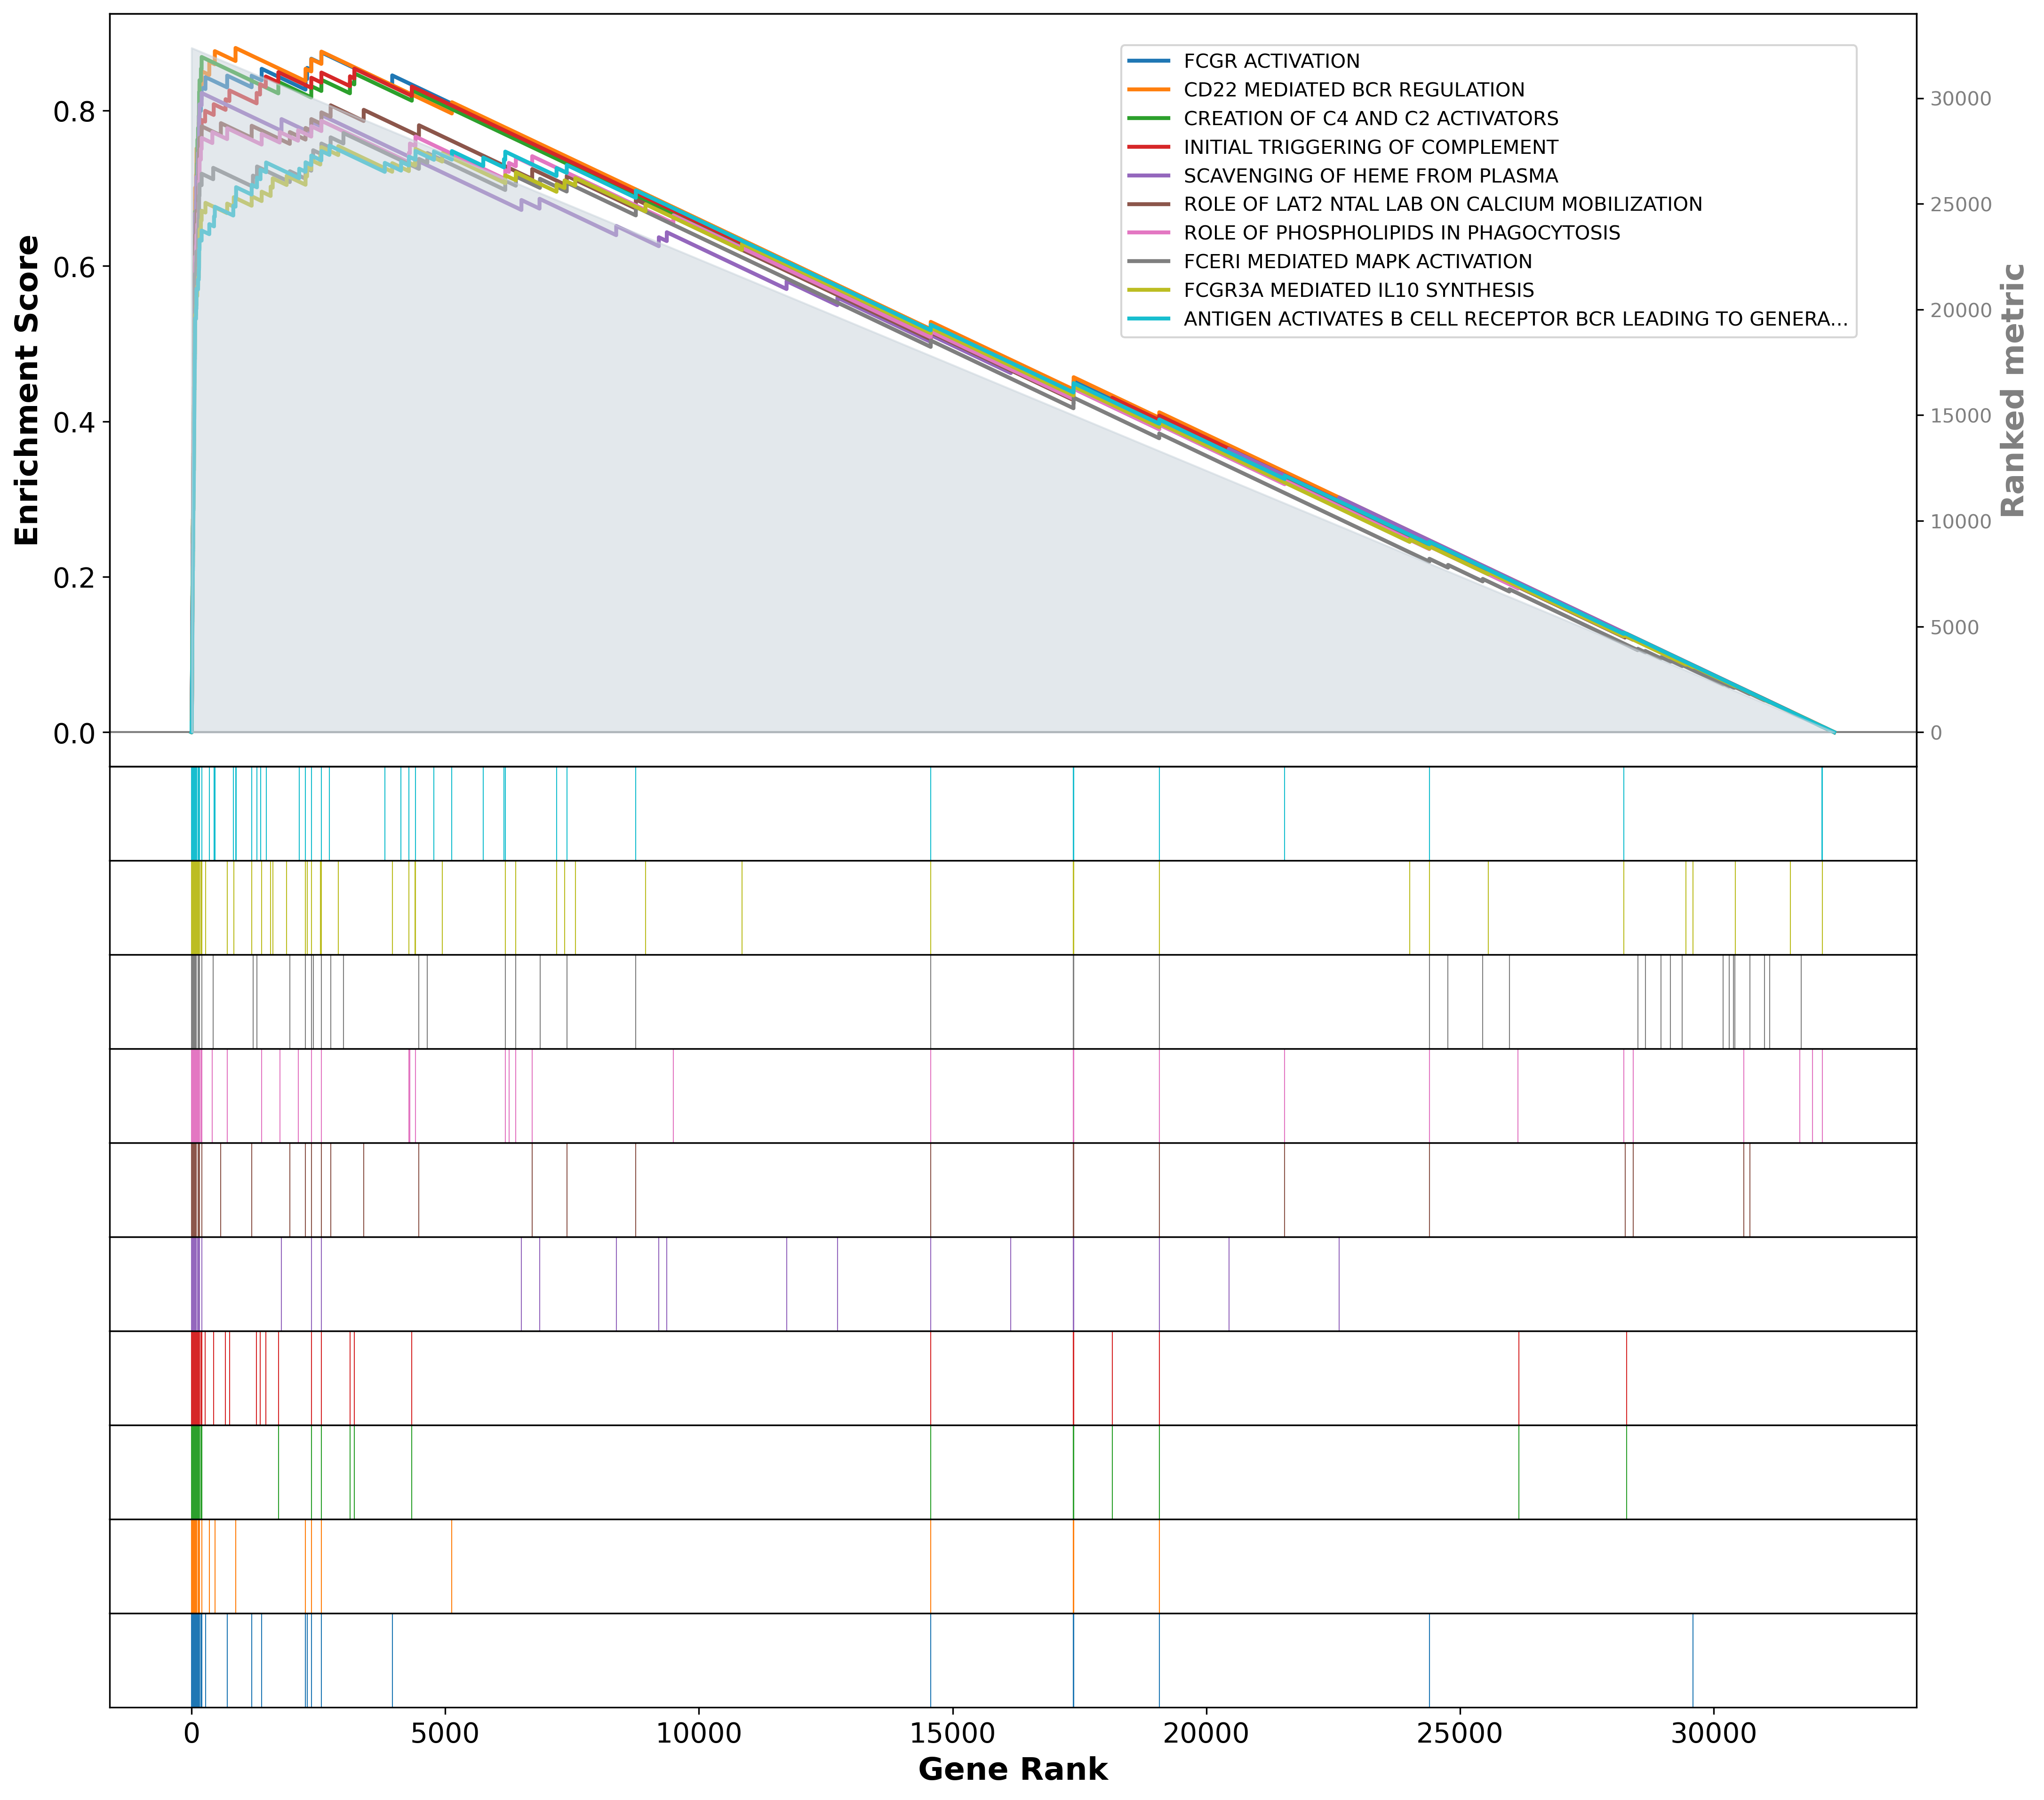
\includegraphics[width=\textwidth, keepaspectratio]{Sections/ClusteringAnalysis/Resources/discussion/other_groups/lumInf_reactome_10_top.png}
        \caption{Top 10 GSEA results on the Reactome database.}
        \label{fig:cs:lumInf_gsea}
    \end{subfigure} 
    \centering
    \caption{Molecular overview of the Luminal Infiltrated (LumInf) group. The Pi plot shows the genes specific to LumInf from the DEA with LowIFNG and LumP, while the GSEA plot displays the top 10 Reactome terms in the enrichment analysis; \acrshort{gsea} was also applied to Hallmarks database in \cref{fig:ap:cs:gsea_lumInf_hallmark} from Appendix.} 
    \label{fig:cs:lumInf}
\end{figure}



\subsubsection{LumP} \label{s:cs:lumP_interp}

The LumInf group exhibits some of the molecular properties of a luminal subtype, but the immune response of the samples is notably strong. In contrast, the tissues from the LumP group are not affected by this 'noise'. To understand the molecular properties of the LumP group, the Pi plot in \cref{fig:cs:lumP_pi} and the \acrshort{gsea} results in \cref{fig:cs:lumP_gsea} are utilised. To highlight the molecular characteristics of the LumP group, \acrshort{dea} between LumP and Ne is performed on the Y-axis, while LumP versus Low IFNG is shown on the X-axis. This configuration ensures that any immune response in LumP is discernible, as both comparison groups are characterised by a lack of immune activity. It also accentuates the markers of the luminal group, given that Low IFNG and Ne possess distinctly different molecular properties.

% LumP specific genes
The points in the first quadrant represent genes specific to the LumP group. It can be seen that there are several sets of genes that are directly associated with bladder differentiation, a trait common to LumP tumours, such as: \textit{PPARG, GATA3, UPK3A, FOXA1}. Other genes significantly expressed in the Luminal Papillary group include \textit{VSIG2, PSCA, ADIRF, DHRS2, SPINK1}. Analysing GO, KEGG pathways and performing DEA between NMIBC and MIBC (microarray dataset \href{https://www.ncbi.nlm.nih.gov/geo/query/acc.cgi?acc=GSE13507}{GSE13507}), the authors in \citet{He2021-de} identified \textit{VSIG2} as one of the three markers for muscle invasiveness. \textit{ADIRF} has been associated with differentiation by work from Lund's group \citet{Eriksson2015-lt}. \textit{DHRS2} protein is highly expressed (see \href{https://www.proteinatlas.org/ENSG00000100867-DHRS2/tissue/urinary+bladder}{Human Protein Atlas}), but is not well studied in the context of MIBC. In the microarray analysis with immunohistochemistry from \citet{Rink2013-sv}, it was found that loss of \textit{SPINK1} was associated with tumour recurrence and aggressiveness.

To further support the non-squamous aspect of the LumP group, some genes that are down-regulated in squamous cell carcinoma (SCC) \citet{Knowles2015-mu} are present in the first quadrant.

% Common between Ne and Low IFNG
In the opposite quadrant, where the genes specific to Ne and Low IFNG are contained, there are markers specific to the Basal (closer to the negative X-axis) such as \textit{KRT6A, KRT6B, KRT14, KRT5}. Additionally, up-regulated SCC markers are near the X-axis, indicating that Low IFNG has stronger SCC markers compared to both the NE and the LumP group. Neuronal markers such as \textit{TUBB2B, GNG4, APLP1} are on the negative side of the Y-axis, denoting the Ne-like aspect over the other two groups in the comparison.

% Explore the genes that are common to both the Low IFNG and NE
In the GSEA plot, the top enriched pathways are down-regulated in the LumP, indicating a strong response from the Ne and Low IFNG groups. The analysis in this subsection highlights the markers for the Luminal groups and reinforces the characteristics of the other two subgroups. It also shows that there are a few genes that are significantly expressed and common to both Low IFNG and NE-like groups. This comparison and the molecular properties of the NE-like group will be further explored in the next subsection.


\begin{figure}[H]
    \centering
    \begin{subfigure}[!t]{1.0\textwidth}
        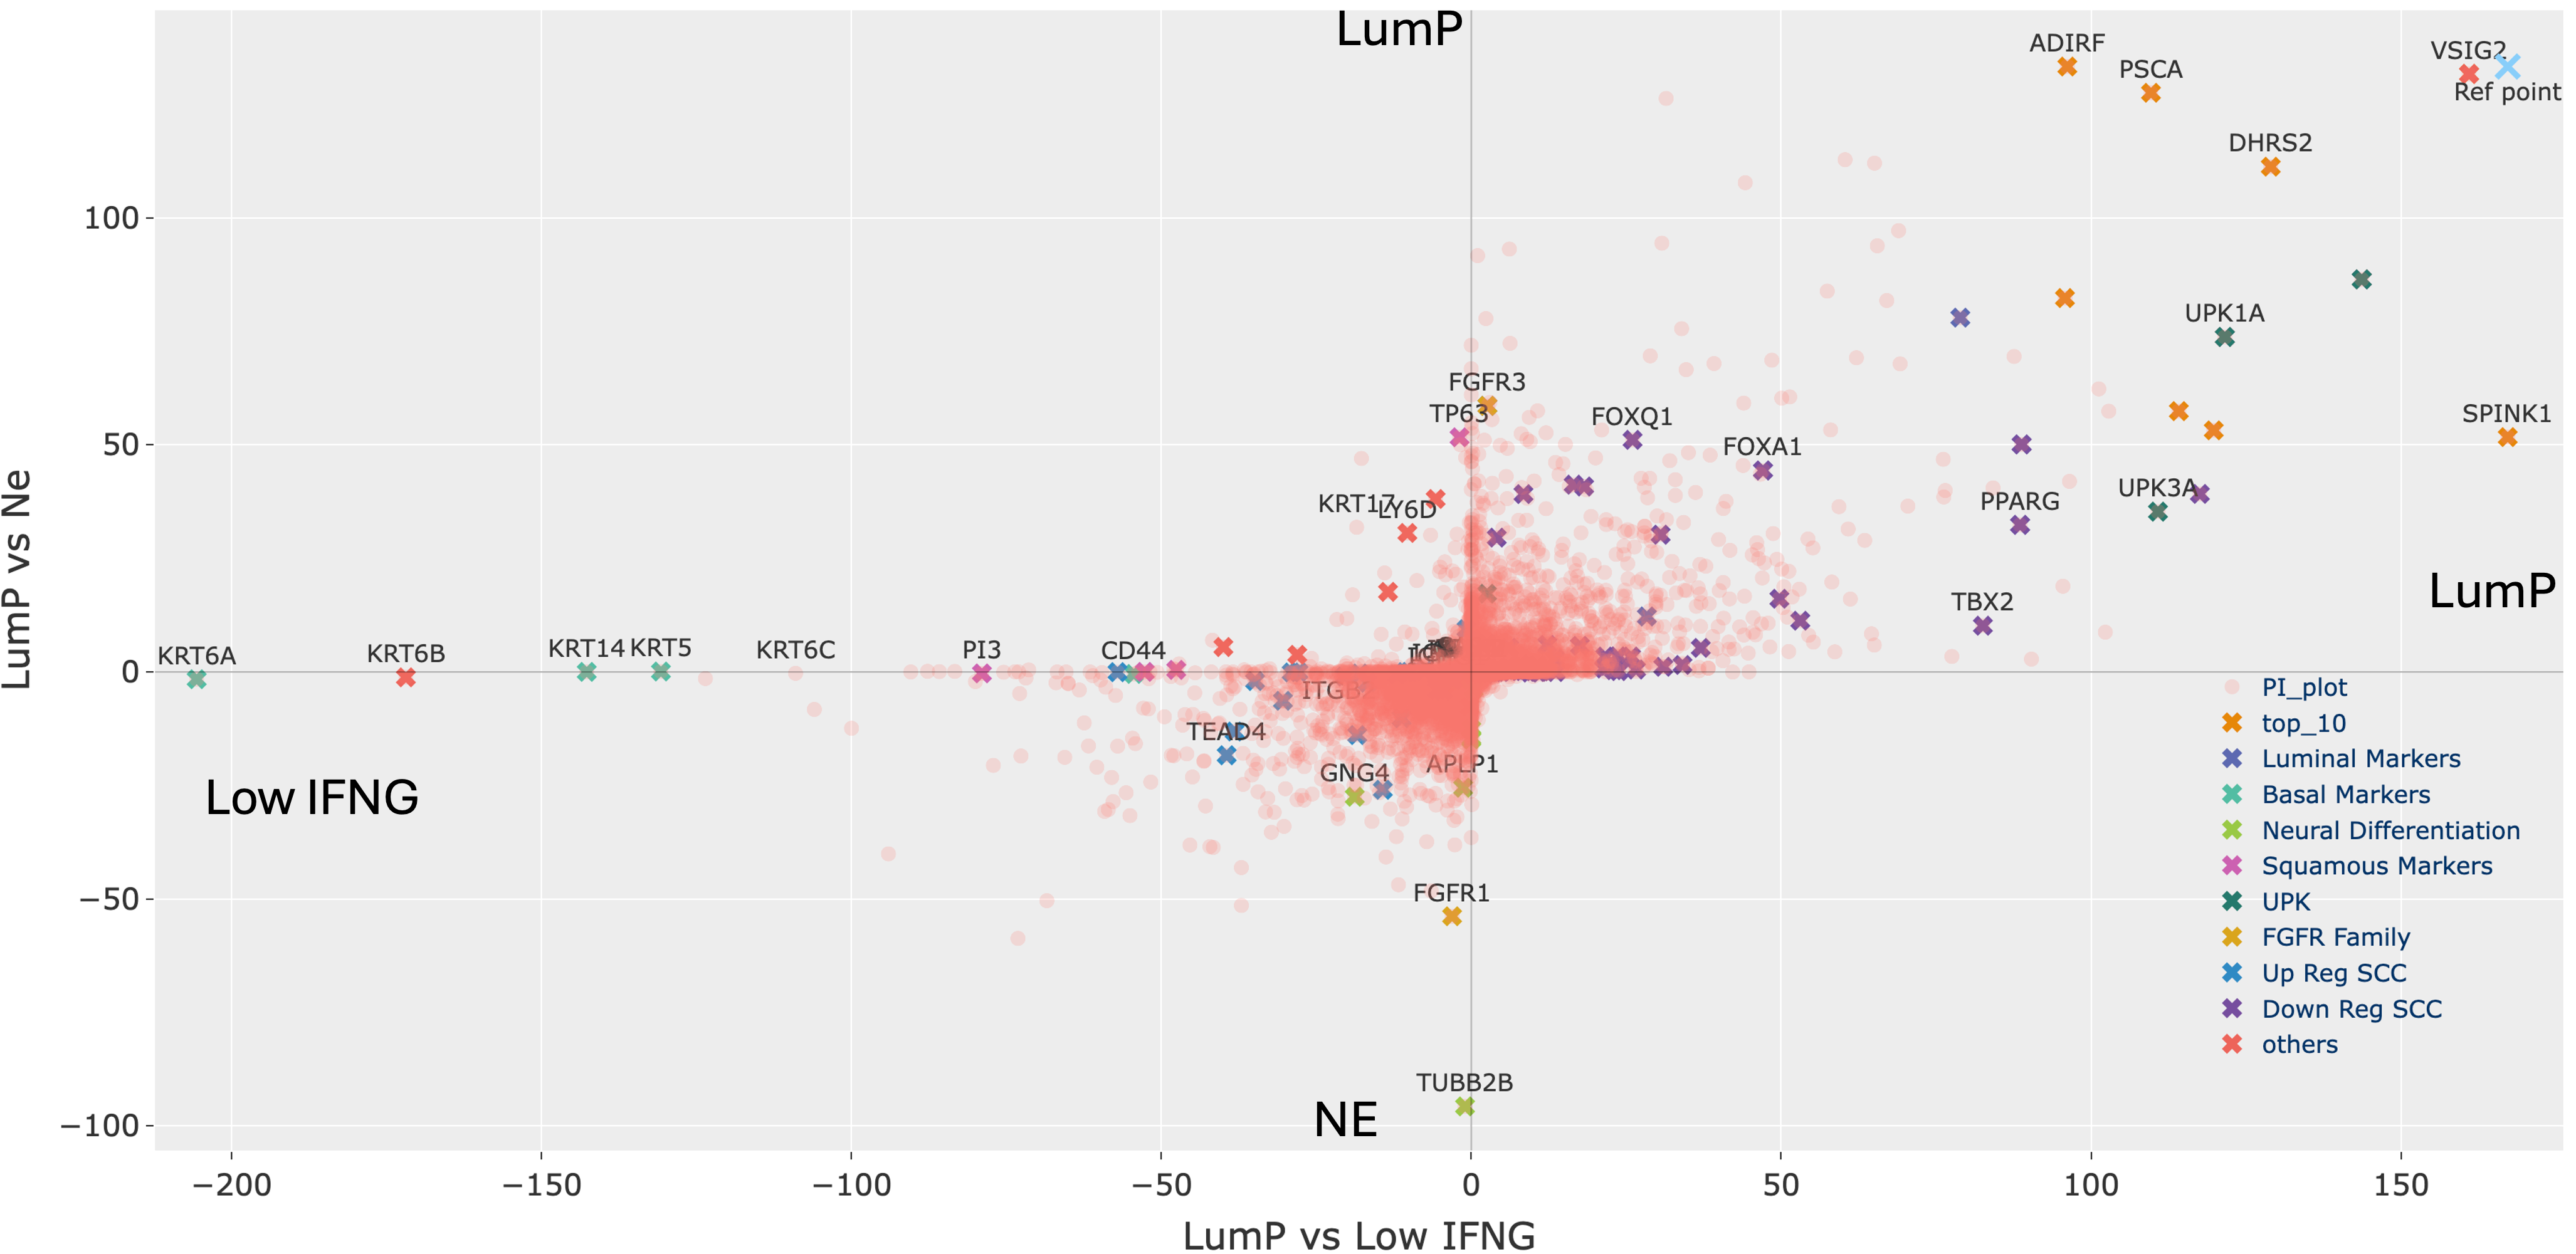
\includegraphics[width=\textwidth,keepaspectratio]{Sections/ClusteringAnalysis/Resources/discussion/other_groups/lump_pi.png}    
        \caption{Pi}
        \label{fig:cs:lumP_pi}
    \end{subfigure}
    \centering
    \begin{subfigure}[!t]{0.91\textwidth}
        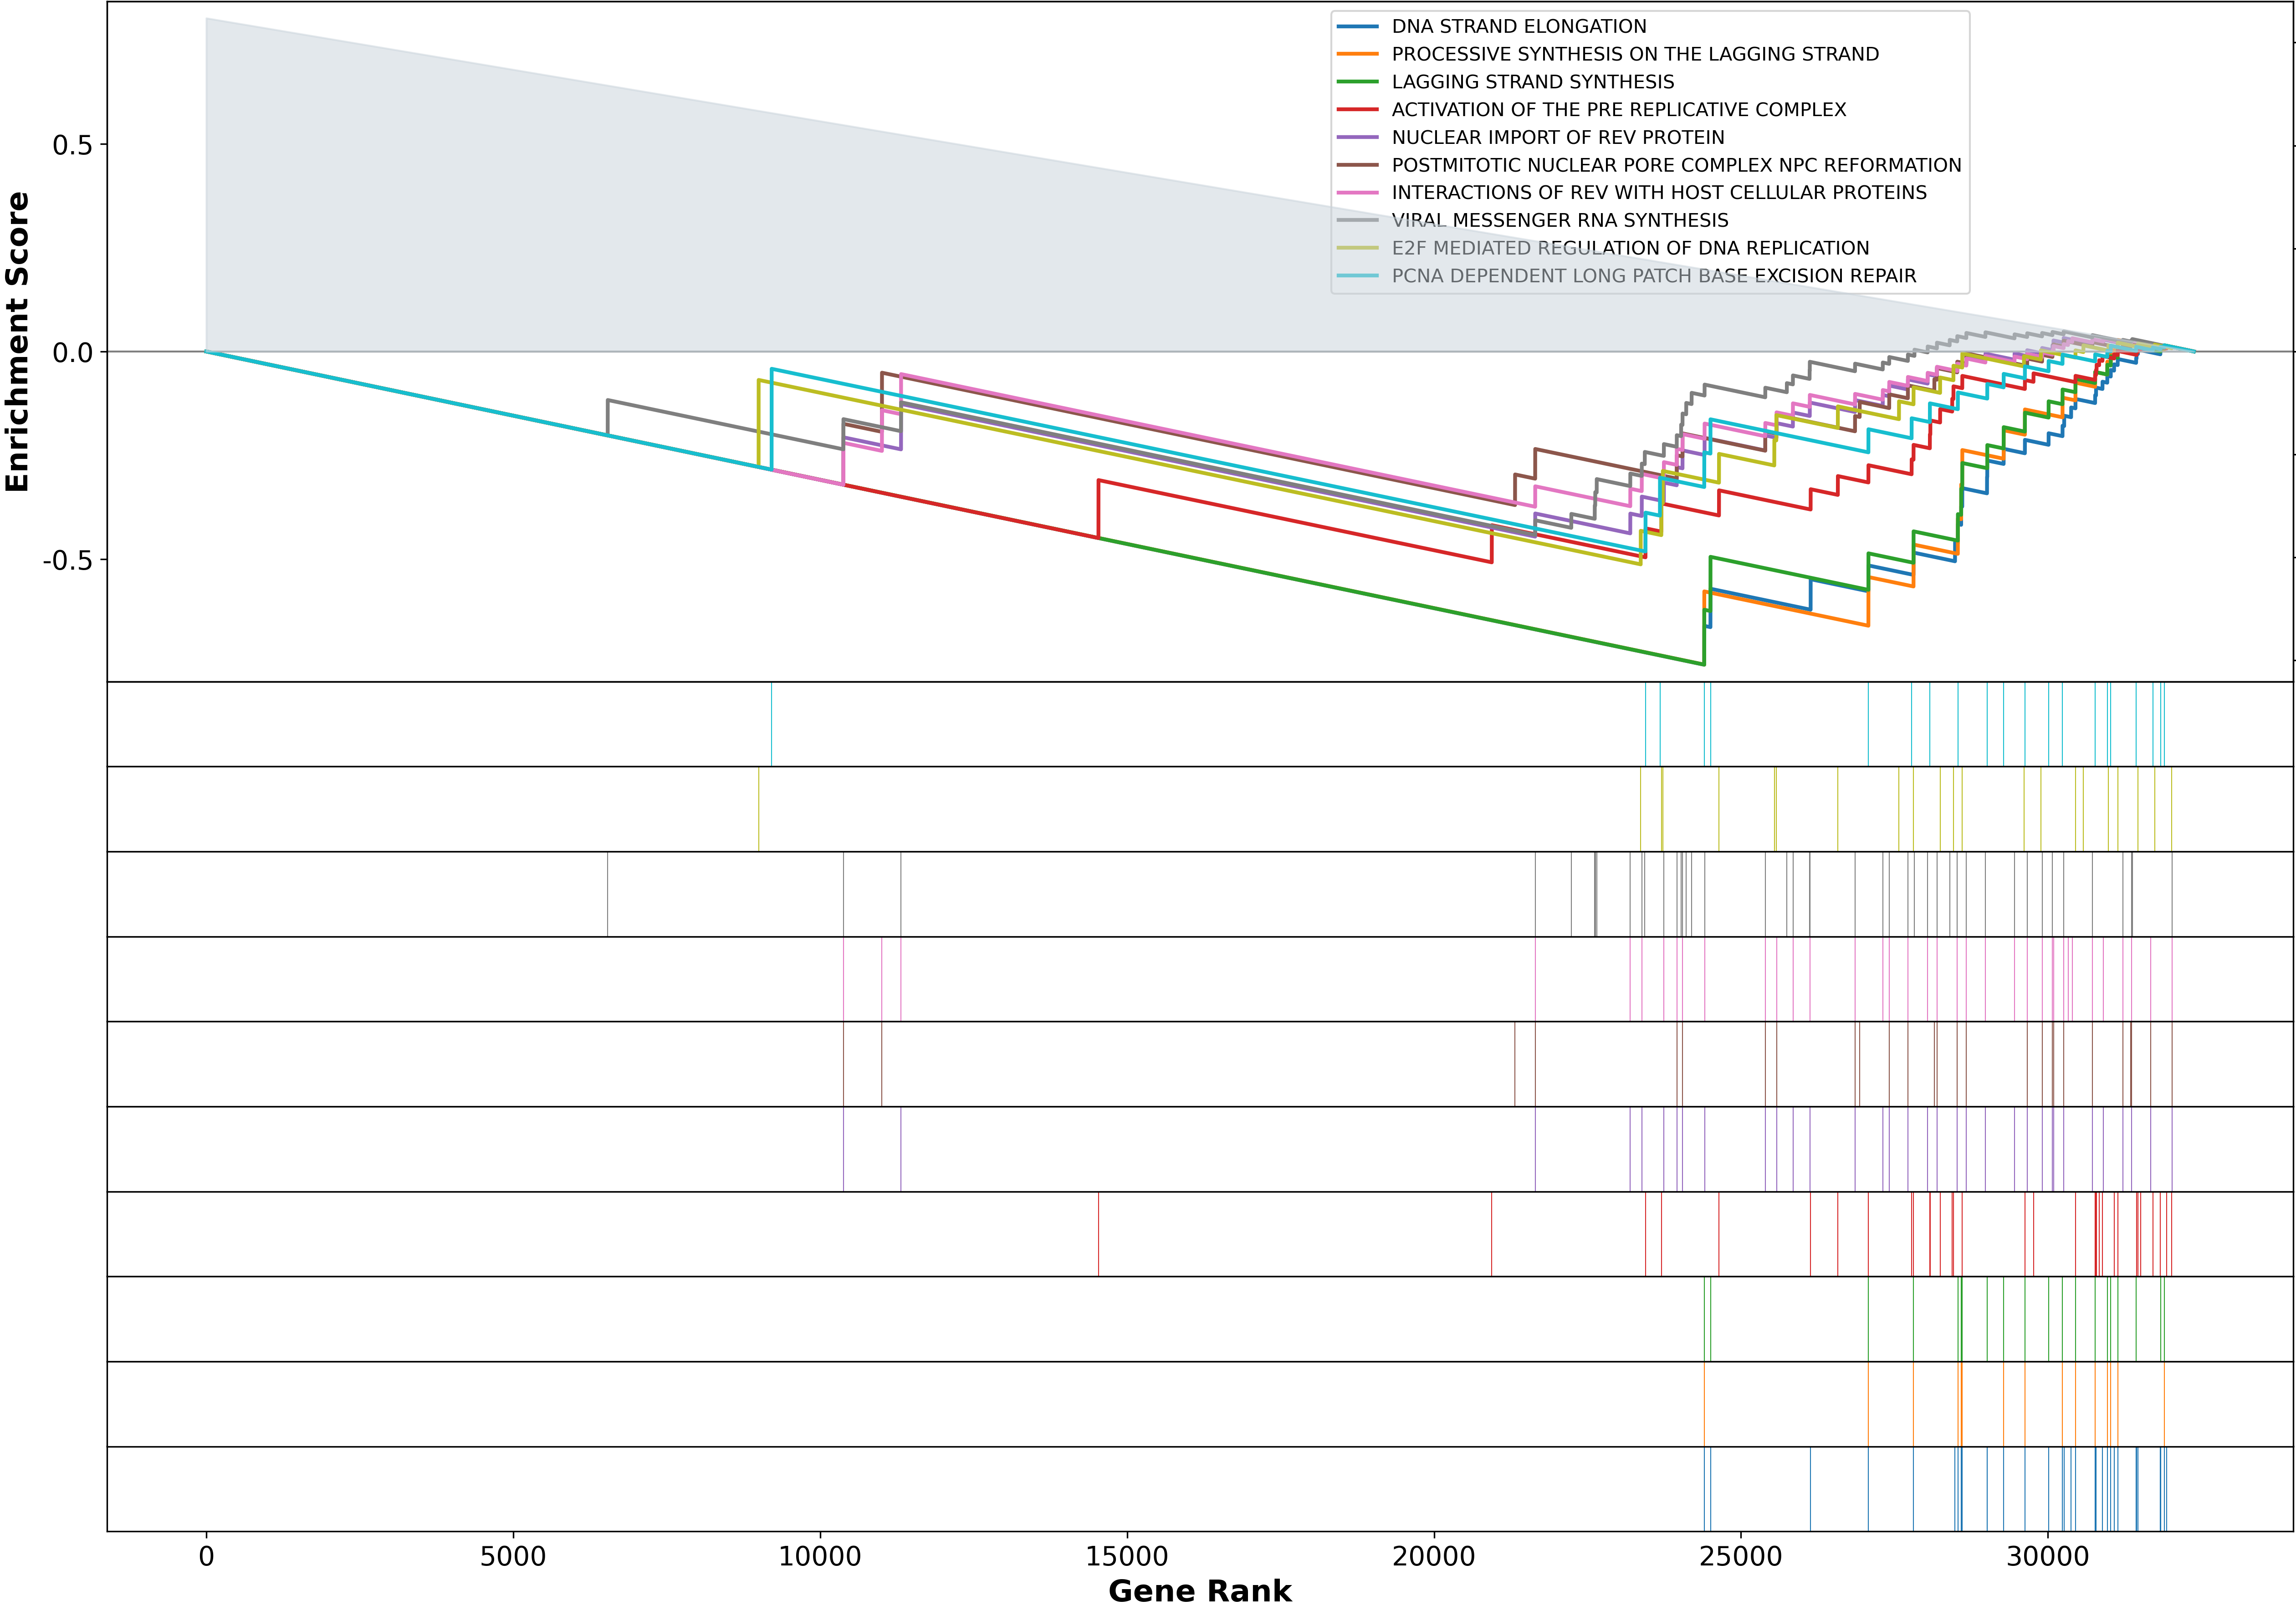
\includegraphics[width=\textwidth, keepaspectratio]{Sections/ClusteringAnalysis/Resources/discussion/other_groups/lumP2_reactome_10_top.png}
        \caption{Top 10 GSEA results on the Reactome database.}
        \label{fig:cs:lumP_gsea}
    \end{subfigure} 
    \centering
    \caption{Molecular overview of the Luminal Papillary (LumP) group. The Pi plot shows the genes specific to LumP from the DEA with Low IFNG and Ne, where the GSEA plot displays the top 10 terms in the enrichment analysis; \acrshort{gsea} was also applied to Hallmarks database in \cref{fig:ap:cs:gsea_lump_hallmark} from Appendix.} 
    \label{fig:cs:lump}
\end{figure}



\subsubsection{NE} \label{s:cs:ne_interp}


In the TCGA's MIBC cohort, the TCGA classifier identified 20 samples as Neuroendocrine like (NE-like), 11 of which are also classified as Sc/NE-like by the Lund classifier, and only 6 of the initial 20 are confirmed as NE-like by the consensus, which includes more than the two datasets mentioned. This suggests that considerable uncertainties still exist regarding the criteria that define the NE group. The clustering analysis conducted in this section grouped \textbf{32} samples into what appears to contain most of the NE-like groups from both the TCGA and Lund datasets \cref{fig:cs:ifn_comp}.

To further explore the NE group derived in this section, the Pi-plot in \cref{fig:cs:ne_pi} displays the \acrshort{dea} comparison of the group with Low IFNG on the Y-axis and with Luminal Papillary on the horizontal axis. These two comparison groups were used as 'representatives' for the Luminal and Basal subtypes as they exhibit the lowest immune infiltration, thus facilitating the observation of any Basal or Luminal tendencies in the NE samples, if present. As can be seen in quadrants I and III \cref{fig:cs:ne_pi}, there are few or no points shared between the studied group and the Basal/Luminal subtypes. This highlights the distinct molecular characteristics of the NE group.

\begin{figure}[!htb]
    \centering
    \begin{subfigure}[!t]{1.0\textwidth}
        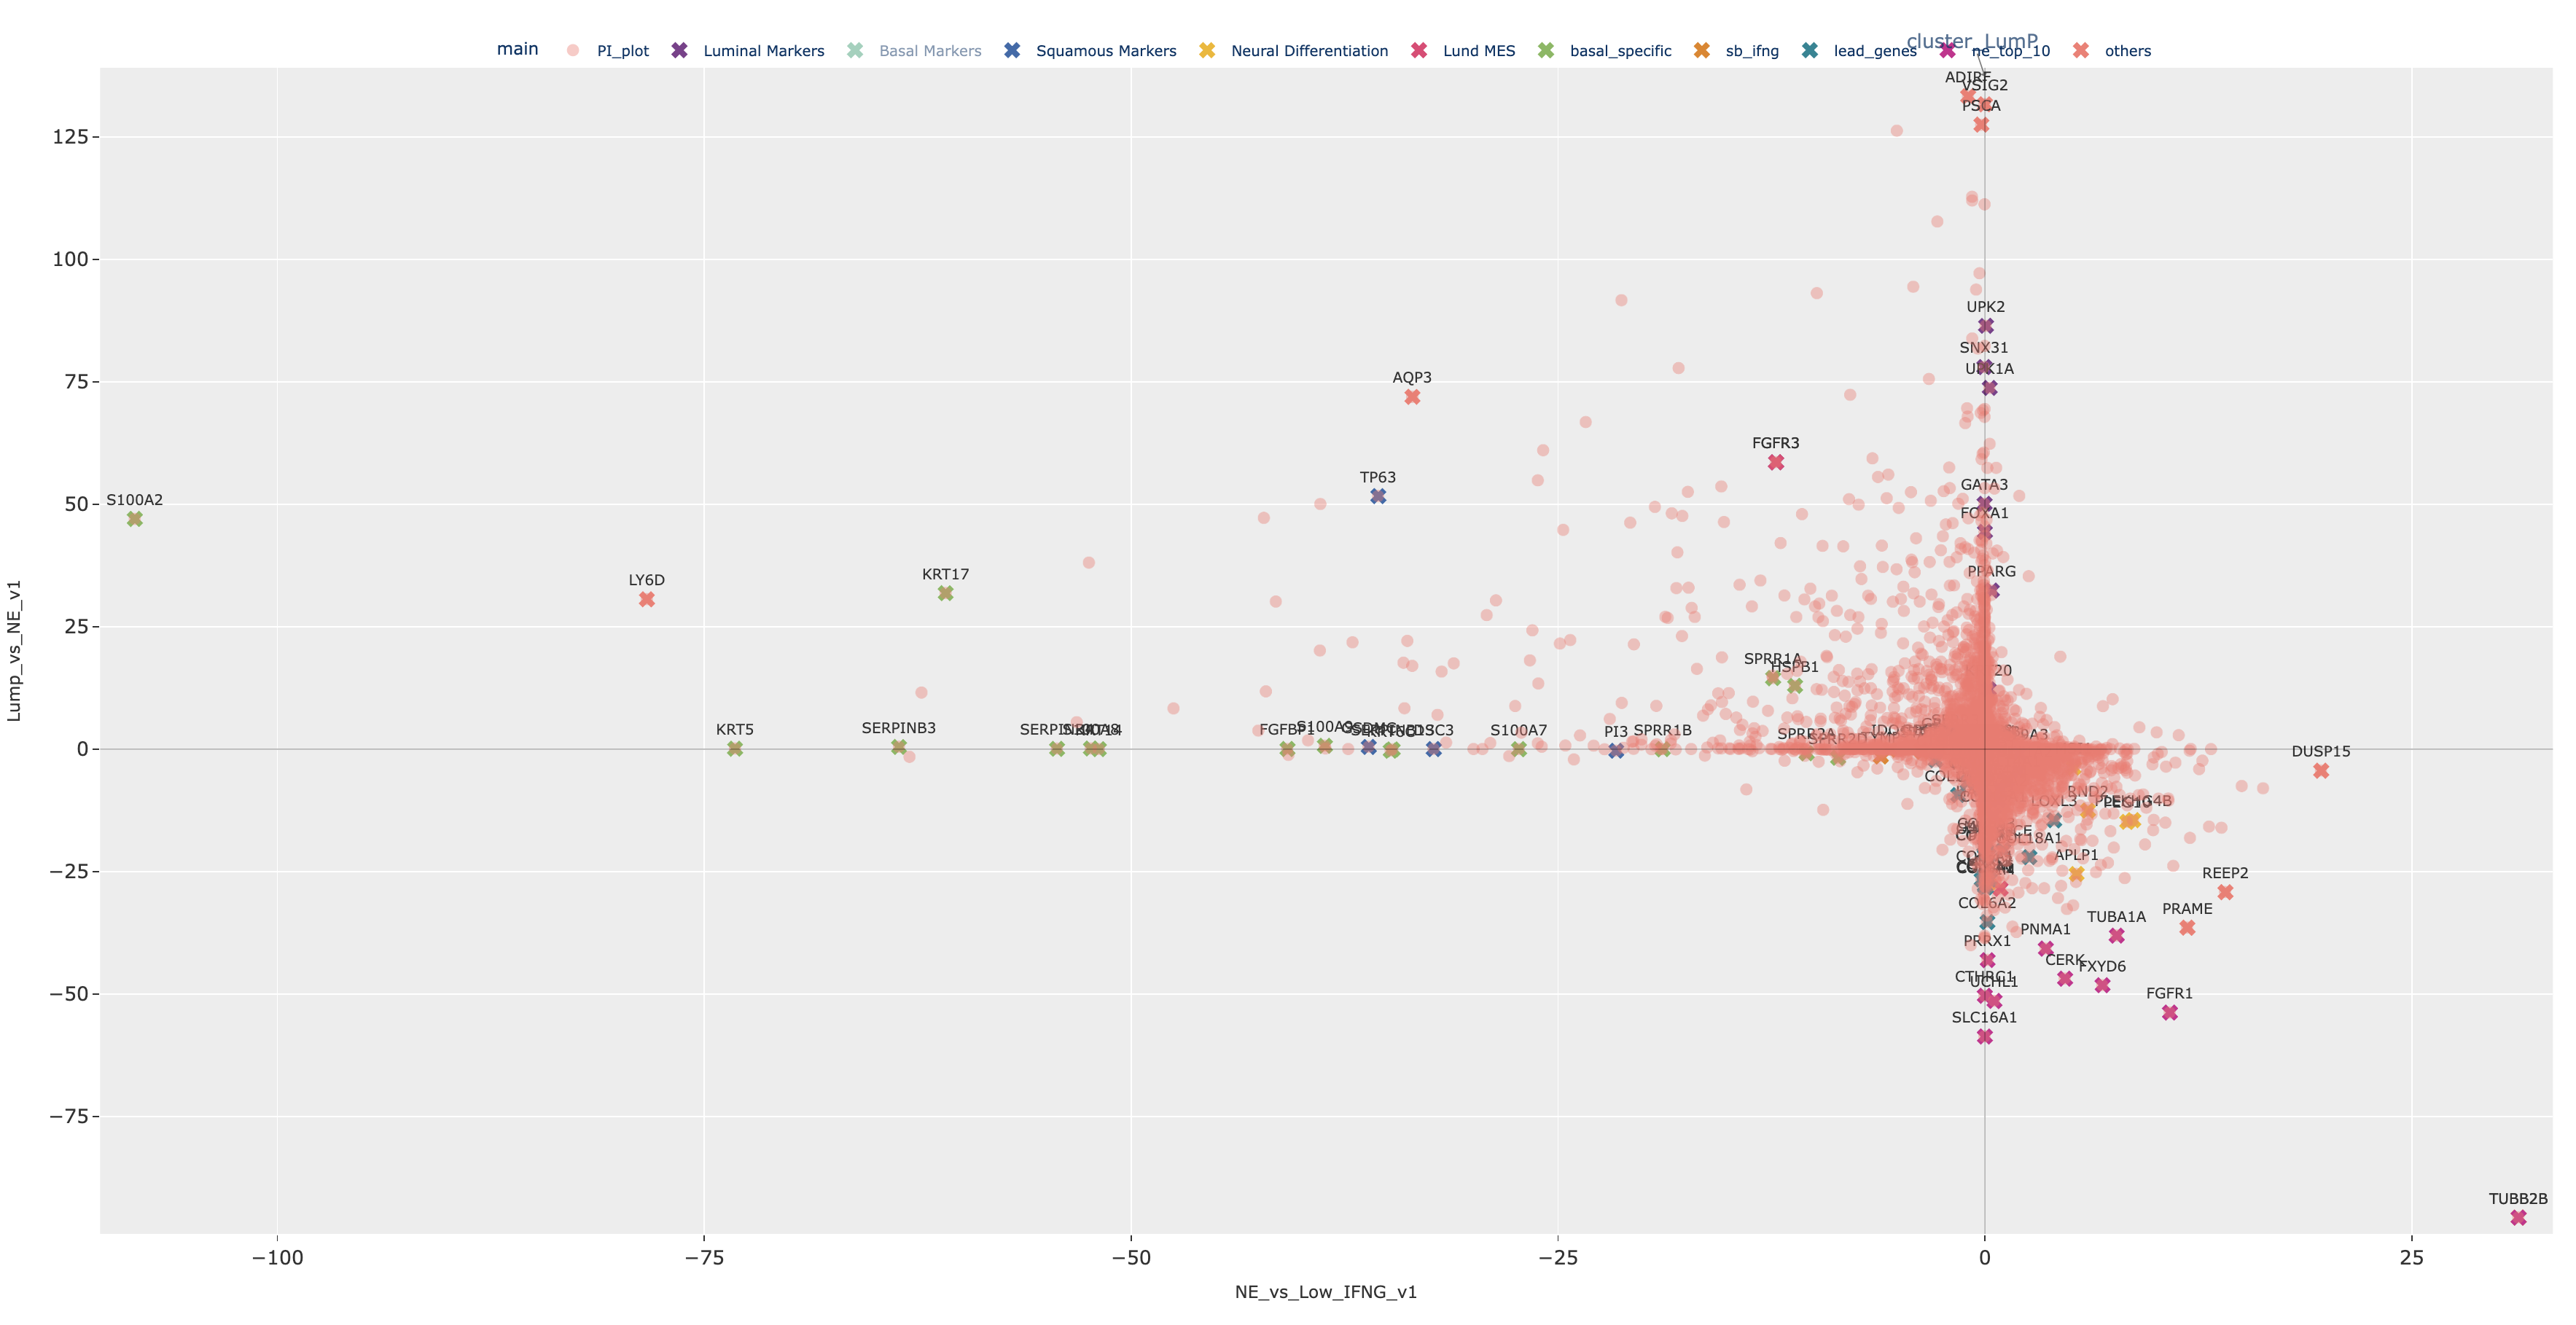
\includegraphics[width=\textwidth,keepaspectratio]{Sections/ClusteringAnalysis/Resources/discussion/other_groups/ne_pi.png}    
        \caption{Pi}
        \label{fig:cs:ne_pi}
    \end{subfigure}
    \centering
    \begin{subfigure}[!t]{0.9\textwidth}
        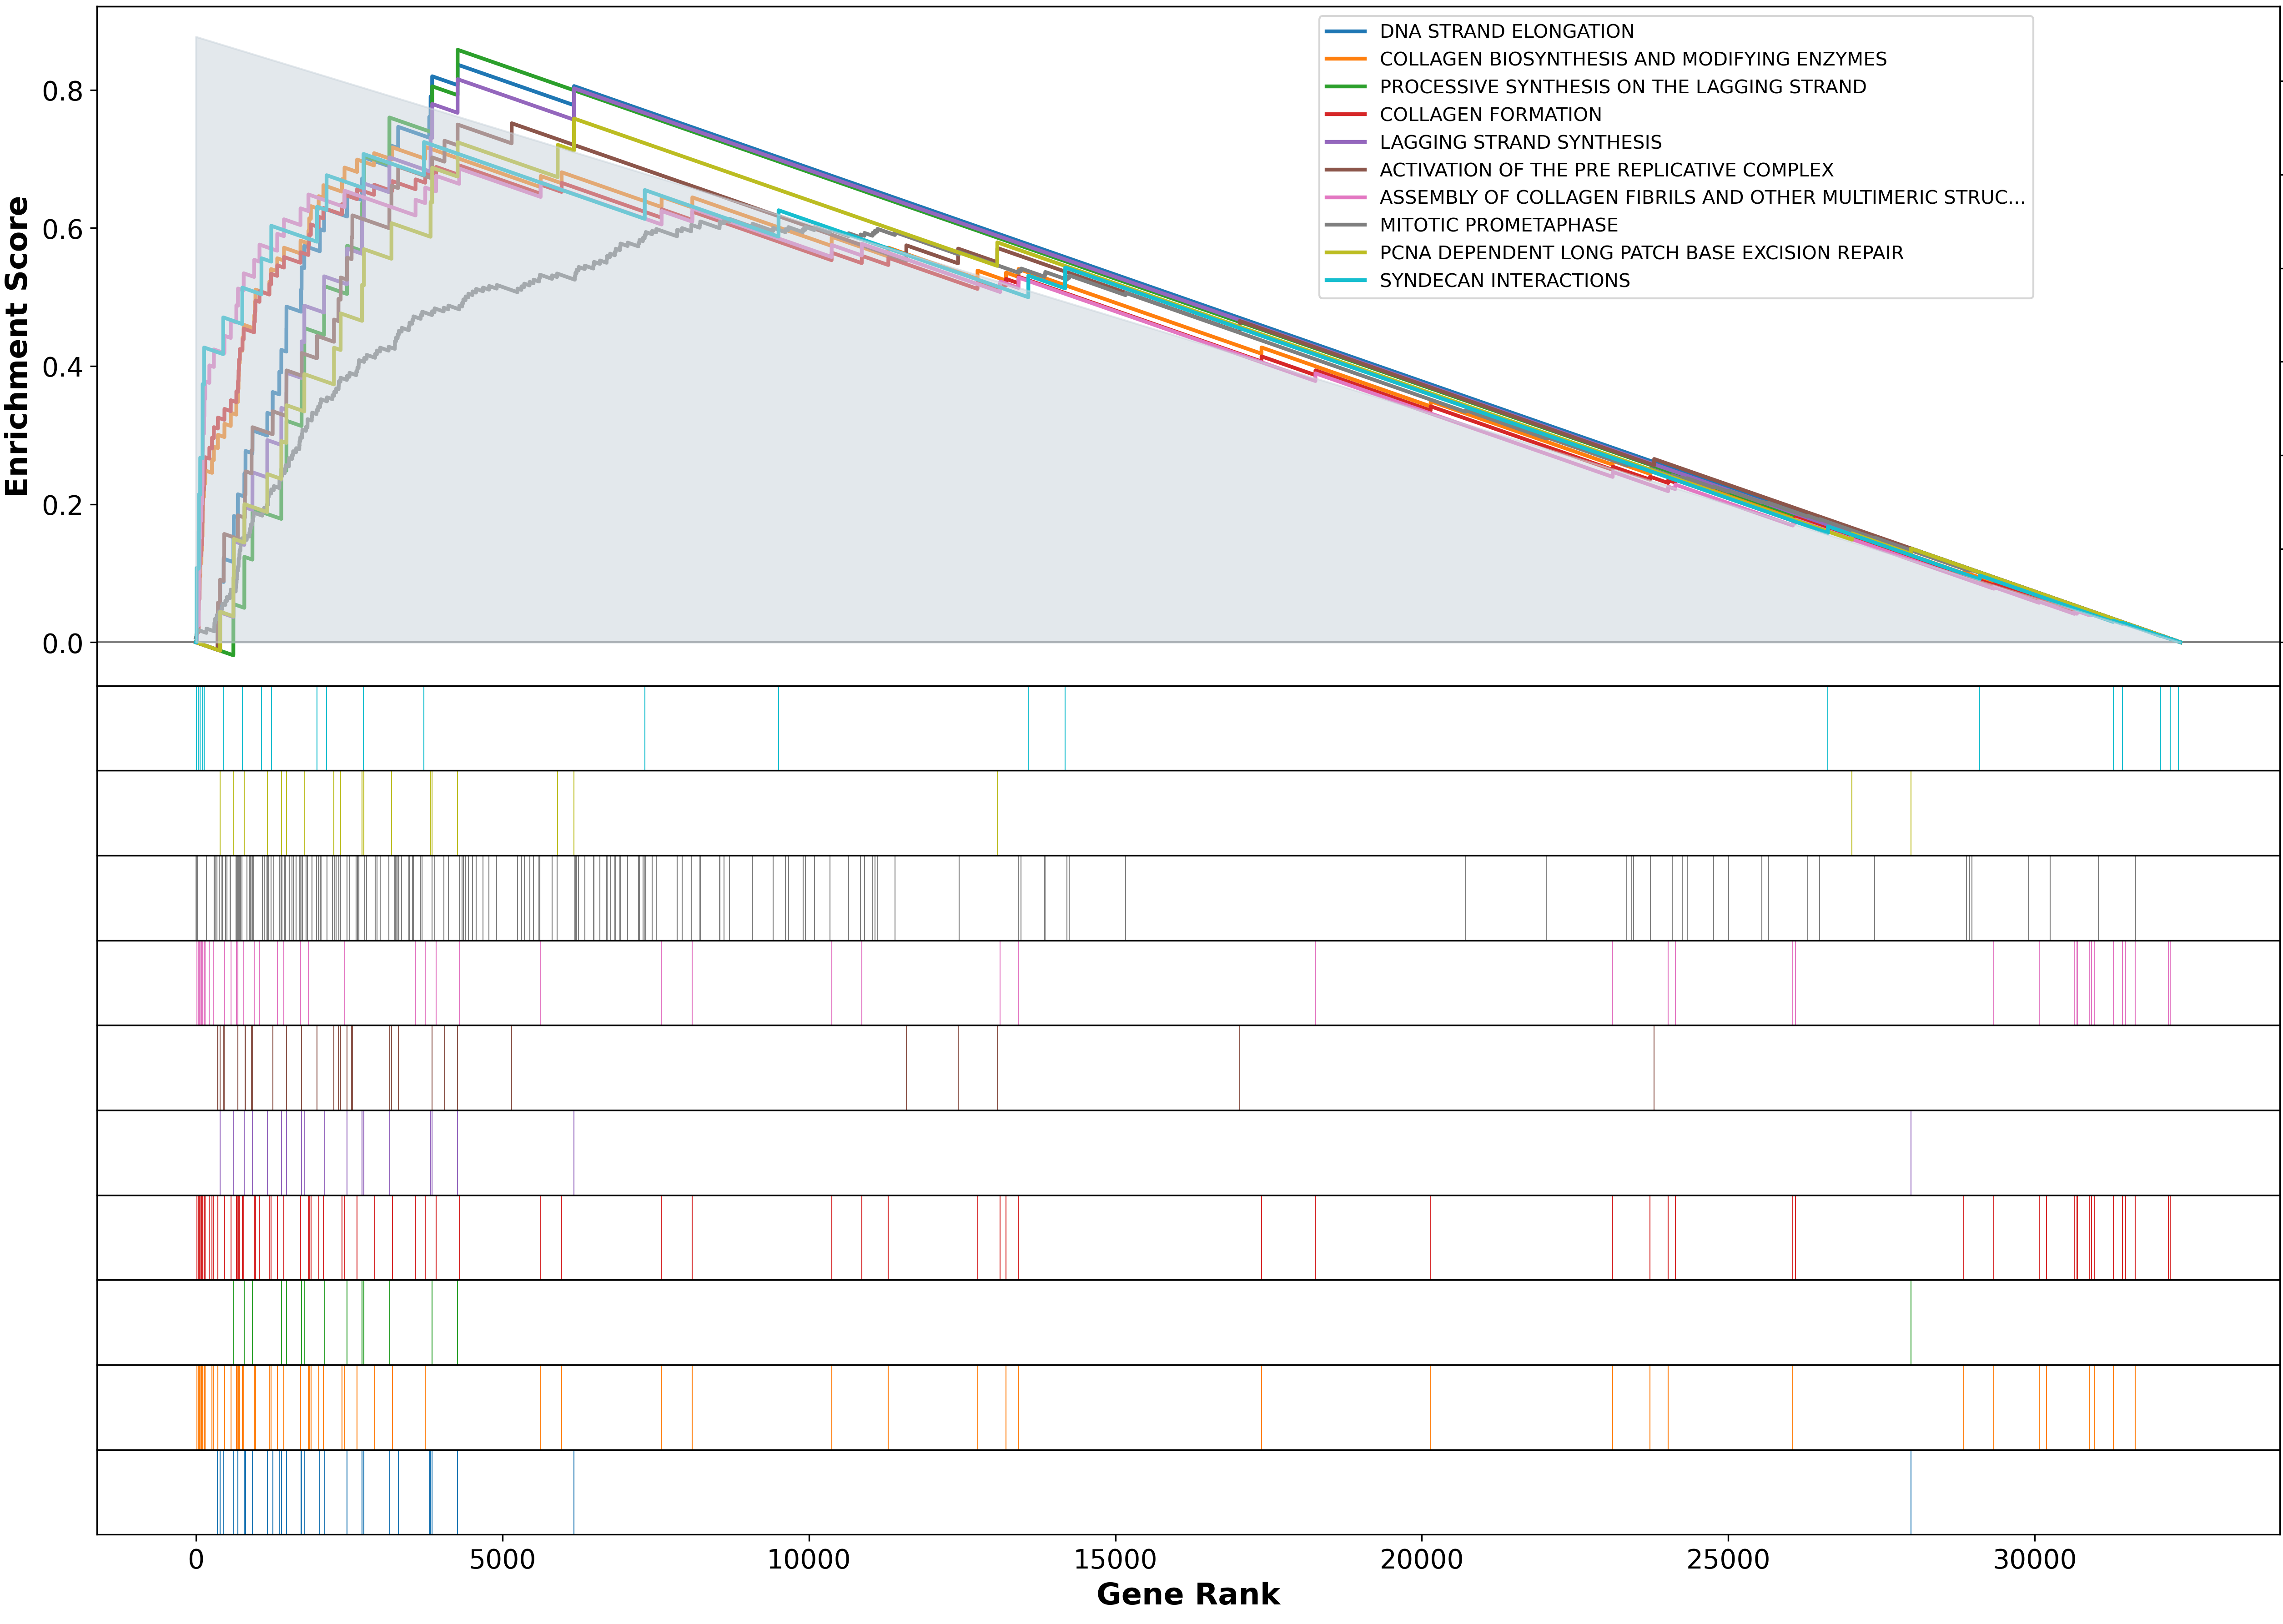
\includegraphics[width=\textwidth, keepaspectratio]{Sections/ClusteringAnalysis/Resources/discussion/other_groups/ne2_reactome_10_top.png}
        \caption{Top 10 GSEA results on the Reactome database.}
        \label{fig:cs:ne_gsea}
    \end{subfigure} 
    \centering
    \caption{Molecular overview of the Neuroendocrine-like (NE) group. The Pi plot displays the genes specific to the NE group from the DEA with Low IFNG and LumP, where the GSEA plot shows the top 10 terms in the enrichment analysis; \acrshort{gsea} was also applied to Hallmarks database in \cref{fig:ap:cs:gsea_ne_hallmark} from Appendix.} 
    \label{fig:cs:ne}
\end{figure}

% Genes associated with the NE
The second quadrant showcases genes specifically associated with the Neuroendocrine like (NE-like) group, including \textit{TUBB2B} and other neuronal markers such as \textit{MSI1, PLEKHG4B, GNG4, PEG10, RND2, APLP1,} and \textit{SOX2} \citep{Robertson2017-mg}. These genes are significantly expressed in the NE-like group, as illustrated by the referential point \cref{fig:cs:ne_pi}, which marks the extremities on the X and Y axes, representing the most pronounced NE-like characteristics from the two comparative analyses. Beyond \textit{TUBB2B}, several genes near this marker hold substantial biological significance, including \textit{TUBA1A, FGFR1, SLC16A1, FXYD6, CTHRC1,} and \textit{PRRX1}.

\textit{TUBA1A}, highly expressed in bladder cancer, has been identified as a potential therapeutic target \citet{Zhang2019-fk} (see \href{https://www.proteinatlas.org/ENSG00000167552-TUBA1A/tissue}{Human Protein Atlas}). \textit{FGFR1}, part of the FGFR family, is associated with cell proliferation, as evidenced in both \textit{in-vitro} and \textit{in-vivo} experiments \citet{Tomlinson2009-td}. \textit{SLC16A1} has been characterised by \citet{Logotheti2020-ya} as a long non-coding gene that enhances cancer invasiveness. \textit{FXYD6}, associated with mental diseases, has shown potential in clinical therapies for a subtype of kidney cancer according to \citet{Gao2014-sq}. In vitro studies suggest \textit{PRRX1} as a therapeutic biomarker for bladder cancer \citet{Huang2022-ez}, with its protein expression being moderately high (see \href{https://www.proteinatlas.org/ENSG00000116132-PRRX1/tissue}{Human Protein Atlas}). Additionally, mouse model research has implicated \textit{CTHRC1} in the proliferation of bladder cancer cells, with high levels correlating with poor prognosis. This protein's high expression is also documented on the \href{https://www.proteinatlas.org/ENSG00000164932-CTHRC1/tissue}{Human Protein Atlas}.

% LumP and Basal
The Low IFNG and LumP comparison groups represent the two major MIBC categories, basal and luminal. The genes in the third quadrant include those common to both groups, while those on the axes are specific to each subtype. On the positive vertical axis, genes such as \textit{UPK2, GATA3, ADIRF, VSIG2} are found, which are known to be associated with tissue differentiation or luminal biology. On the horizontal axis, basal-specific markers are displayed, such as \textit{KRT5} and the SERP family. \textit{AQP3, TP64, FGFR3} are highlighted in the scatter plot as markers known to be expressed across MIBC tumours.

% GSEA
The GSEA plot in \cref{fig:cs:ne_gsea} reveals several pathways related to collagen or the lagging strand, suggesting the involvement of these genes in Epithelial Mesenchymal Transition (EMT). This is emphasized by the GSEA run on the Hallmark database, presented in the Appendix \cref{fig:ap:cs:gsea_ne_hallmark}, which also identifies pathways involved in the cell cycle. The analysis of the NE quadrant highlights the neuronal nature of the subgroups but also underlines the potential to discover new genes specific to the subtype. Overall, the analysis shows that the studied group exhibits gene expression patterns distinct from those of the luminal and basal groups.
